\documentclass[12pt]{article}
\usepackage[letterpaper, top=22mm, bottom=20mm, left=15mm, right=15mm, headheight=15pt, headsep=6mm, footskip=10mm]{geometry}
\usepackage[T1]{fontenc}
\usepackage{tgheros}
\renewcommand{\familydefault}{\sfdefault}
\usepackage{tikz}
\usetikzlibrary{arrows.meta}
\usepackage{fancyhdr}
\pagestyle{fancy}
\fancyhf{}
\renewcommand{\headrulewidth}{0pt}
\fancyhead[L]{Week 91 / Rotor-router machines / K--1}
\fancyfoot[L]{\small Bellingham Math Circle / Week 91 / F91-K-v1}
\fancyfoot[R]{\small \thepage}
\setlength{\parindent}{0pt}
\setlength{\parskip}{0pt}
\linespread{1.15}
\newcommand{\problem}[2]{\par\noindent\textbf{Problem #1:} #2\par}
\begin{document}
Before the first counter, clear the exits and point each card the way you choose.
Copy the starting arrows with spare cards beside the board.
A counter starts beside the top card and always waits beside a card, never on top of it.
At each card it moves where the arrow points, and then that card is flipped.
One counter reaches an exit before the next one starts.
The board's cards change only by flipping.

\vspace{6mm}
\begin{center}
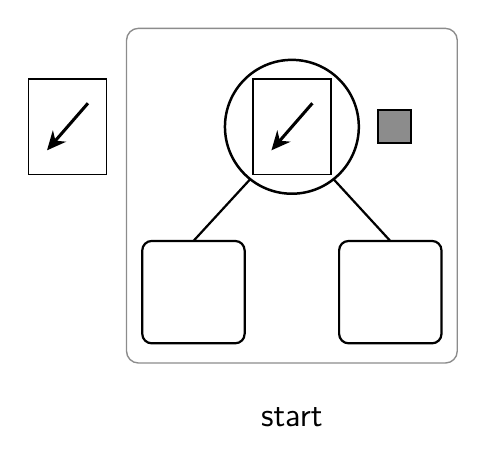
\begin{tikzpicture}[x=1mm,y=1mm,baseline=0]
\draw[line width=0.5pt, black!45, rounded corners=1.5mm] (-21,12.5) rectangle (21,-30);
\draw[line width=0.9pt] (0,0) circle (8.5);
\draw[line width=0.6pt, fill=white] (-4.95,-6.05) rectangle (4.95,6.05);
\draw[-{Stealth[length=2.4mm,width=2.2mm]}, line width=1.1pt] (2.60,2.99) -- (-2.60,-2.99);
\draw[line width=0.6pt, fill=white] (-33.45,-6.05) rectangle (-23.55,6.05);
\draw[-{Stealth[length=2.4mm,width=2.2mm]}, line width=1.1pt] (-25.90,2.99) -- (-31.10,-2.99);
\draw[line width=0.8pt] (-5.27,-6.63) -- (-12.50,-14.50);
\draw[line width=0.8pt, rounded corners=1.2mm] (-19.00,-27.50) rectangle (-6.00,-14.50);
\draw[line width=0.8pt] (5.27,-6.63) -- (12.50,-14.50);
\draw[line width=0.8pt, rounded corners=1.2mm] (6.00,-27.50) rectangle (19.00,-14.50);
\filldraw[fill=black!45, draw=black, line width=0.6pt] (10.90,-2.10) rectangle (15.10,2.10);
\node[font=\large, anchor=base] at (0,-38) {start};
\end{tikzpicture}\hspace{9mm}
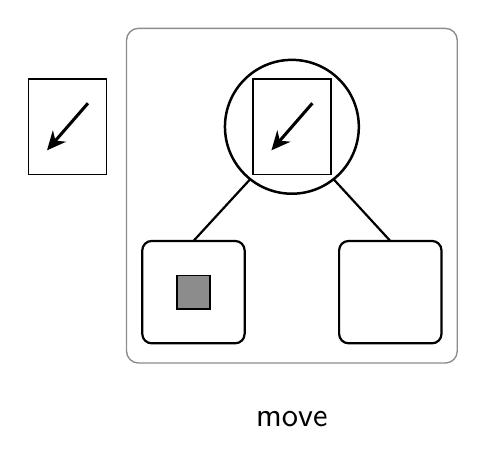
\begin{tikzpicture}[x=1mm,y=1mm,baseline=0]
\draw[line width=0.5pt, black!45, rounded corners=1.5mm] (-21,12.5) rectangle (21,-30);
\draw[line width=0.9pt] (0,0) circle (8.5);
\draw[line width=0.6pt, fill=white] (-4.95,-6.05) rectangle (4.95,6.05);
\draw[-{Stealth[length=2.4mm,width=2.2mm]}, line width=1.1pt] (2.60,2.99) -- (-2.60,-2.99);
\draw[line width=0.6pt, fill=white] (-33.45,-6.05) rectangle (-23.55,6.05);
\draw[-{Stealth[length=2.4mm,width=2.2mm]}, line width=1.1pt] (-25.90,2.99) -- (-31.10,-2.99);
\draw[line width=0.8pt] (-5.27,-6.63) -- (-12.50,-14.50);
\draw[line width=0.8pt, rounded corners=1.2mm] (-19.00,-27.50) rectangle (-6.00,-14.50);
\draw[line width=0.8pt] (5.27,-6.63) -- (12.50,-14.50);
\draw[line width=0.8pt, rounded corners=1.2mm] (6.00,-27.50) rectangle (19.00,-14.50);
\filldraw[fill=black!45, draw=black, line width=0.6pt] (-14.60,-23.10) rectangle (-10.40,-18.90);
\node[font=\large, anchor=base] at (0,-38) {move};
\end{tikzpicture}\hspace{9mm}
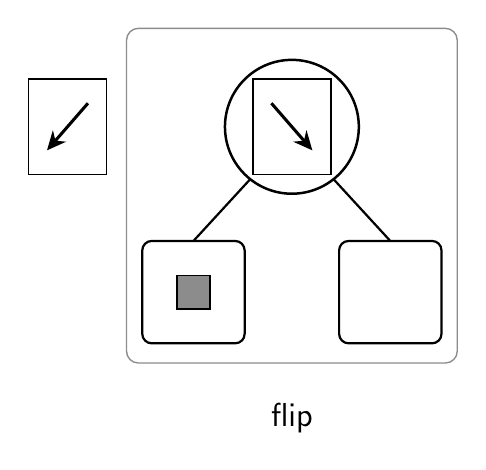
\begin{tikzpicture}[x=1mm,y=1mm,baseline=0]
\draw[line width=0.5pt, black!45, rounded corners=1.5mm] (-21,12.5) rectangle (21,-30);
\draw[line width=0.9pt] (0,0) circle (8.5);
\draw[line width=0.6pt, fill=white] (-4.95,-6.05) rectangle (4.95,6.05);
\draw[-{Stealth[length=2.4mm,width=2.2mm]}, line width=1.1pt] (-2.60,2.99) -- (2.60,-2.99);
\draw[line width=0.6pt, fill=white] (-33.45,-6.05) rectangle (-23.55,6.05);
\draw[-{Stealth[length=2.4mm,width=2.2mm]}, line width=1.1pt] (-25.90,2.99) -- (-31.10,-2.99);
\draw[line width=0.8pt] (-5.27,-6.63) -- (-12.50,-14.50);
\draw[line width=0.8pt, rounded corners=1.2mm] (-19.00,-27.50) rectangle (-6.00,-14.50);
\draw[line width=0.8pt] (5.27,-6.63) -- (12.50,-14.50);
\draw[line width=0.8pt, rounded corners=1.2mm] (6.00,-27.50) rectangle (19.00,-14.50);
\filldraw[fill=black!45, draw=black, line width=0.6pt] (-14.60,-23.10) rectangle (-10.40,-18.90);
\node[font=\large, anchor=base] at (0,-38) {flip};
\end{tikzpicture}
\end{center}
\vspace{6mm}
\problem{1}{Set the card on the board with exits X and Y and send 10 counters, writing where each one lands. Can two counters in a row land on the same exit?}
\vspace{8mm}
\begin{center}
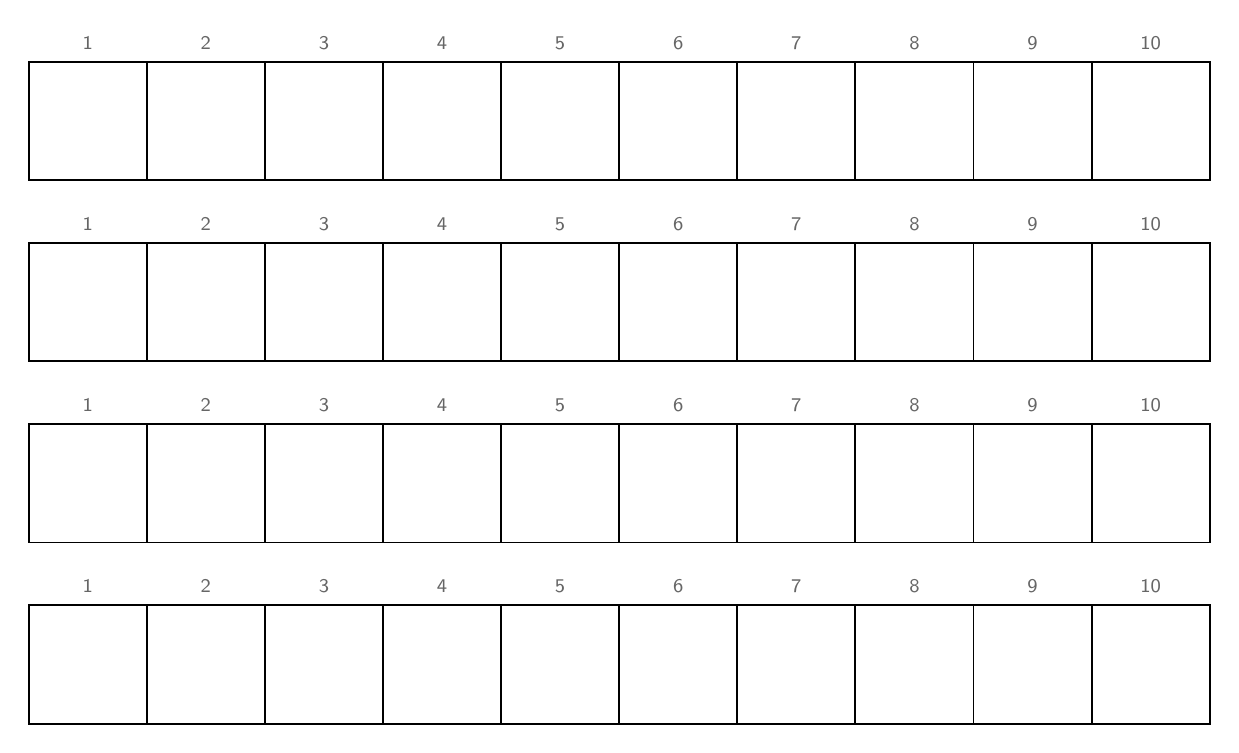
\begin{tikzpicture}[x=1mm,y=1mm,baseline=0]
\draw[line width=0.7pt] (0,0) rectangle (15,-15);
\node[font=\scriptsize, text=black!60] at (7.5,2.4) {1};
\draw[line width=0.7pt] (15,0) rectangle (30,-15);
\node[font=\scriptsize, text=black!60] at (22.5,2.4) {2};
\draw[line width=0.7pt] (30,0) rectangle (45,-15);
\node[font=\scriptsize, text=black!60] at (37.5,2.4) {3};
\draw[line width=0.7pt] (45,0) rectangle (60,-15);
\node[font=\scriptsize, text=black!60] at (52.5,2.4) {4};
\draw[line width=0.7pt] (60,0) rectangle (75,-15);
\node[font=\scriptsize, text=black!60] at (67.5,2.4) {5};
\draw[line width=0.7pt] (75,0) rectangle (90,-15);
\node[font=\scriptsize, text=black!60] at (82.5,2.4) {6};
\draw[line width=0.7pt] (90,0) rectangle (105,-15);
\node[font=\scriptsize, text=black!60] at (97.5,2.4) {7};
\draw[line width=0.7pt] (105,0) rectangle (120,-15);
\node[font=\scriptsize, text=black!60] at (112.5,2.4) {8};
\draw[line width=0.7pt] (120,0) rectangle (135,-15);
\node[font=\scriptsize, text=black!60] at (127.5,2.4) {9};
\draw[line width=0.7pt] (135,0) rectangle (150,-15);
\node[font=\scriptsize, text=black!60] at (142.5,2.4) {10};
\draw[line width=0.7pt] (0,-23) rectangle (15,-38);
\node[font=\scriptsize, text=black!60] at (7.5,-20.6) {1};
\draw[line width=0.7pt] (15,-23) rectangle (30,-38);
\node[font=\scriptsize, text=black!60] at (22.5,-20.6) {2};
\draw[line width=0.7pt] (30,-23) rectangle (45,-38);
\node[font=\scriptsize, text=black!60] at (37.5,-20.6) {3};
\draw[line width=0.7pt] (45,-23) rectangle (60,-38);
\node[font=\scriptsize, text=black!60] at (52.5,-20.6) {4};
\draw[line width=0.7pt] (60,-23) rectangle (75,-38);
\node[font=\scriptsize, text=black!60] at (67.5,-20.6) {5};
\draw[line width=0.7pt] (75,-23) rectangle (90,-38);
\node[font=\scriptsize, text=black!60] at (82.5,-20.6) {6};
\draw[line width=0.7pt] (90,-23) rectangle (105,-38);
\node[font=\scriptsize, text=black!60] at (97.5,-20.6) {7};
\draw[line width=0.7pt] (105,-23) rectangle (120,-38);
\node[font=\scriptsize, text=black!60] at (112.5,-20.6) {8};
\draw[line width=0.7pt] (120,-23) rectangle (135,-38);
\node[font=\scriptsize, text=black!60] at (127.5,-20.6) {9};
\draw[line width=0.7pt] (135,-23) rectangle (150,-38);
\node[font=\scriptsize, text=black!60] at (142.5,-20.6) {10};
\draw[line width=0.7pt] (0,-46) rectangle (15,-61);
\node[font=\scriptsize, text=black!60] at (7.5,-43.6) {1};
\draw[line width=0.7pt] (15,-46) rectangle (30,-61);
\node[font=\scriptsize, text=black!60] at (22.5,-43.6) {2};
\draw[line width=0.7pt] (30,-46) rectangle (45,-61);
\node[font=\scriptsize, text=black!60] at (37.5,-43.6) {3};
\draw[line width=0.7pt] (45,-46) rectangle (60,-61);
\node[font=\scriptsize, text=black!60] at (52.5,-43.6) {4};
\draw[line width=0.7pt] (60,-46) rectangle (75,-61);
\node[font=\scriptsize, text=black!60] at (67.5,-43.6) {5};
\draw[line width=0.7pt] (75,-46) rectangle (90,-61);
\node[font=\scriptsize, text=black!60] at (82.5,-43.6) {6};
\draw[line width=0.7pt] (90,-46) rectangle (105,-61);
\node[font=\scriptsize, text=black!60] at (97.5,-43.6) {7};
\draw[line width=0.7pt] (105,-46) rectangle (120,-61);
\node[font=\scriptsize, text=black!60] at (112.5,-43.6) {8};
\draw[line width=0.7pt] (120,-46) rectangle (135,-61);
\node[font=\scriptsize, text=black!60] at (127.5,-43.6) {9};
\draw[line width=0.7pt] (135,-46) rectangle (150,-61);
\node[font=\scriptsize, text=black!60] at (142.5,-43.6) {10};
\draw[line width=0.7pt] (0,-69) rectangle (15,-84);
\node[font=\scriptsize, text=black!60] at (7.5,-66.6) {1};
\draw[line width=0.7pt] (15,-69) rectangle (30,-84);
\node[font=\scriptsize, text=black!60] at (22.5,-66.6) {2};
\draw[line width=0.7pt] (30,-69) rectangle (45,-84);
\node[font=\scriptsize, text=black!60] at (37.5,-66.6) {3};
\draw[line width=0.7pt] (45,-69) rectangle (60,-84);
\node[font=\scriptsize, text=black!60] at (52.5,-66.6) {4};
\draw[line width=0.7pt] (60,-69) rectangle (75,-84);
\node[font=\scriptsize, text=black!60] at (67.5,-66.6) {5};
\draw[line width=0.7pt] (75,-69) rectangle (90,-84);
\node[font=\scriptsize, text=black!60] at (82.5,-66.6) {6};
\draw[line width=0.7pt] (90,-69) rectangle (105,-84);
\node[font=\scriptsize, text=black!60] at (97.5,-66.6) {7};
\draw[line width=0.7pt] (105,-69) rectangle (120,-84);
\node[font=\scriptsize, text=black!60] at (112.5,-66.6) {8};
\draw[line width=0.7pt] (120,-69) rectangle (135,-84);
\node[font=\scriptsize, text=black!60] at (127.5,-66.6) {9};
\draw[line width=0.7pt] (135,-69) rectangle (150,-84);
\node[font=\scriptsize, text=black!60] at (142.5,-66.6) {10};
\end{tikzpicture}
\end{center}
\newpage
\problem{2}{Make the piles in each picture on the X and Y board, and draw the starting arrow that makes them. Cross out any picture that no starting arrow can make.}
\vspace{18mm}
\noindent 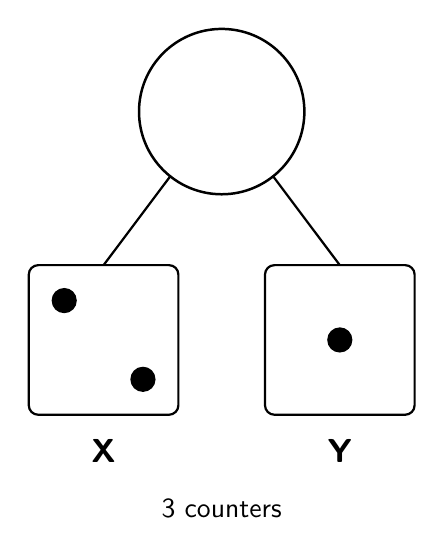
\begin{tikzpicture}[x=1mm,y=1mm,baseline=0]
\draw[line width=0.9pt] (0,0) circle (10.5);
\draw[line width=0.8pt] (-6.51,-8.19) -- (-15.00,-19.50);
\draw[line width=0.8pt, rounded corners=1.2mm] (-24.50,-38.50) rectangle (-5.50,-19.50);
\node[font=\bfseries\large] at (-15.00,-43.10) {X};
\fill (-20.00,-24.00) circle (1.6);\fill (-10.00,-34.00) circle (1.6);
\draw[line width=0.8pt] (6.51,-8.19) -- (15.00,-19.50);
\draw[line width=0.8pt, rounded corners=1.2mm] (5.50,-38.50) rectangle (24.50,-19.50);
\node[font=\bfseries\large] at (15.00,-43.10) {Y};
\fill (15.00,-29.00) circle (1.6);
\node[font=\normalsize, anchor=base] at (0,-51.50) {3 counters};
\end{tikzpicture}
\hfill
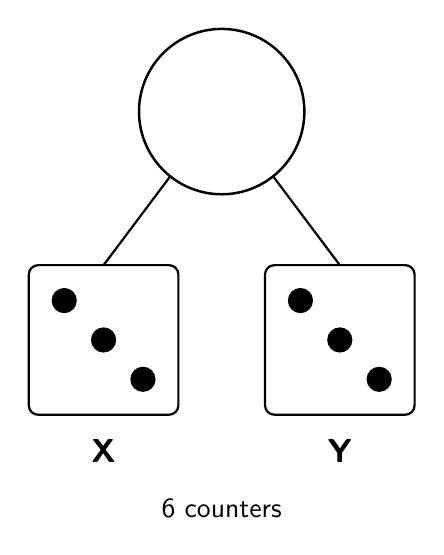
\begin{tikzpicture}[x=1mm,y=1mm,baseline=0]
\draw[line width=0.9pt] (0,0) circle (10.5);
\draw[line width=0.8pt] (-6.51,-8.19) -- (-15.00,-19.50);
\draw[line width=0.8pt, rounded corners=1.2mm] (-24.50,-38.50) rectangle (-5.50,-19.50);
\node[font=\bfseries\large] at (-15.00,-43.10) {X};
\fill (-20.00,-24.00) circle (1.6);\fill (-15.00,-29.00) circle (1.6);\fill (-10.00,-34.00) circle (1.6);
\draw[line width=0.8pt] (6.51,-8.19) -- (15.00,-19.50);
\draw[line width=0.8pt, rounded corners=1.2mm] (5.50,-38.50) rectangle (24.50,-19.50);
\node[font=\bfseries\large] at (15.00,-43.10) {Y};
\fill (10.00,-24.00) circle (1.6);\fill (15.00,-29.00) circle (1.6);\fill (20.00,-34.00) circle (1.6);
\node[font=\normalsize, anchor=base] at (0,-51.50) {6 counters};
\end{tikzpicture}
\hfill
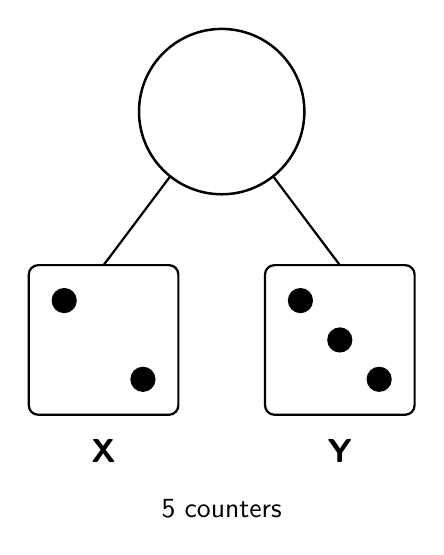
\begin{tikzpicture}[x=1mm,y=1mm,baseline=0]
\draw[line width=0.9pt] (0,0) circle (10.5);
\draw[line width=0.8pt] (-6.51,-8.19) -- (-15.00,-19.50);
\draw[line width=0.8pt, rounded corners=1.2mm] (-24.50,-38.50) rectangle (-5.50,-19.50);
\node[font=\bfseries\large] at (-15.00,-43.10) {X};
\fill (-20.00,-24.00) circle (1.6);\fill (-10.00,-34.00) circle (1.6);
\draw[line width=0.8pt] (6.51,-8.19) -- (15.00,-19.50);
\draw[line width=0.8pt, rounded corners=1.2mm] (5.50,-38.50) rectangle (24.50,-19.50);
\node[font=\bfseries\large] at (15.00,-43.10) {Y};
\fill (10.00,-24.00) circle (1.6);\fill (15.00,-29.00) circle (1.6);\fill (20.00,-34.00) circle (1.6);
\node[font=\normalsize, anchor=base] at (0,-51.50) {5 counters};
\end{tikzpicture}

\vspace{26mm}
\noindent 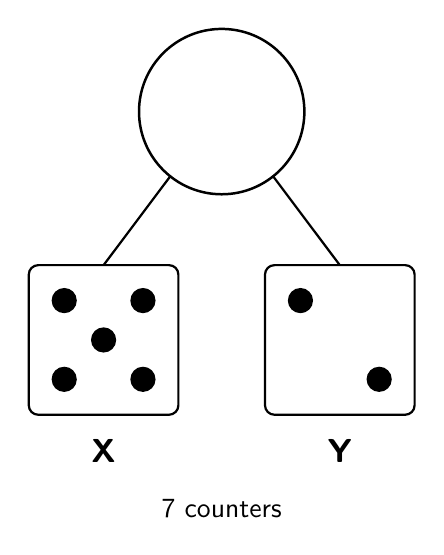
\begin{tikzpicture}[x=1mm,y=1mm,baseline=0]
\draw[line width=0.9pt] (0,0) circle (10.5);
\draw[line width=0.8pt] (-6.51,-8.19) -- (-15.00,-19.50);
\draw[line width=0.8pt, rounded corners=1.2mm] (-24.50,-38.50) rectangle (-5.50,-19.50);
\node[font=\bfseries\large] at (-15.00,-43.10) {X};
\fill (-20.00,-24.00) circle (1.6);\fill (-10.00,-24.00) circle (1.6);\fill (-15.00,-29.00) circle (1.6);\fill (-20.00,-34.00) circle (1.6);\fill (-10.00,-34.00) circle (1.6);
\draw[line width=0.8pt] (6.51,-8.19) -- (15.00,-19.50);
\draw[line width=0.8pt, rounded corners=1.2mm] (5.50,-38.50) rectangle (24.50,-19.50);
\node[font=\bfseries\large] at (15.00,-43.10) {Y};
\fill (10.00,-24.00) circle (1.6);\fill (20.00,-34.00) circle (1.6);
\node[font=\normalsize, anchor=base] at (0,-51.50) {7 counters};
\end{tikzpicture}
\hfill
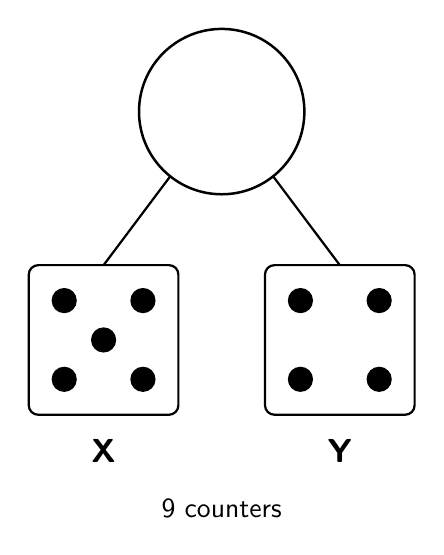
\begin{tikzpicture}[x=1mm,y=1mm,baseline=0]
\draw[line width=0.9pt] (0,0) circle (10.5);
\draw[line width=0.8pt] (-6.51,-8.19) -- (-15.00,-19.50);
\draw[line width=0.8pt, rounded corners=1.2mm] (-24.50,-38.50) rectangle (-5.50,-19.50);
\node[font=\bfseries\large] at (-15.00,-43.10) {X};
\fill (-20.00,-24.00) circle (1.6);\fill (-10.00,-24.00) circle (1.6);\fill (-15.00,-29.00) circle (1.6);\fill (-20.00,-34.00) circle (1.6);\fill (-10.00,-34.00) circle (1.6);
\draw[line width=0.8pt] (6.51,-8.19) -- (15.00,-19.50);
\draw[line width=0.8pt, rounded corners=1.2mm] (5.50,-38.50) rectangle (24.50,-19.50);
\node[font=\bfseries\large] at (15.00,-43.10) {Y};
\fill (10.00,-24.00) circle (1.6);\fill (20.00,-24.00) circle (1.6);\fill (10.00,-34.00) circle (1.6);\fill (20.00,-34.00) circle (1.6);
\node[font=\normalsize, anchor=base] at (0,-51.50) {9 counters};
\end{tikzpicture}
\hfill
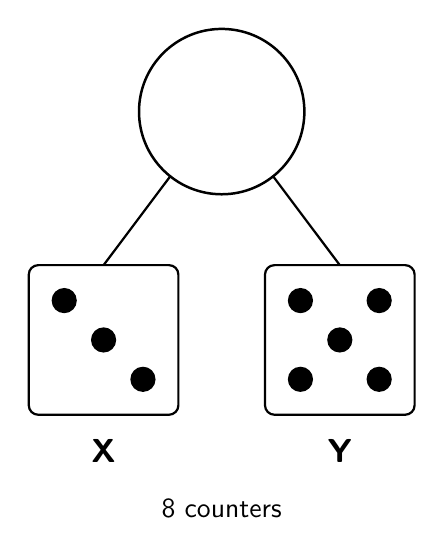
\begin{tikzpicture}[x=1mm,y=1mm,baseline=0]
\draw[line width=0.9pt] (0,0) circle (10.5);
\draw[line width=0.8pt] (-6.51,-8.19) -- (-15.00,-19.50);
\draw[line width=0.8pt, rounded corners=1.2mm] (-24.50,-38.50) rectangle (-5.50,-19.50);
\node[font=\bfseries\large] at (-15.00,-43.10) {X};
\fill (-20.00,-24.00) circle (1.6);\fill (-15.00,-29.00) circle (1.6);\fill (-10.00,-34.00) circle (1.6);
\draw[line width=0.8pt] (6.51,-8.19) -- (15.00,-19.50);
\draw[line width=0.8pt, rounded corners=1.2mm] (5.50,-38.50) rectangle (24.50,-19.50);
\node[font=\bfseries\large] at (15.00,-43.10) {Y};
\fill (10.00,-24.00) circle (1.6);\fill (20.00,-24.00) circle (1.6);\fill (15.00,-29.00) circle (1.6);\fill (10.00,-34.00) circle (1.6);\fill (20.00,-34.00) circle (1.6);
\node[font=\normalsize, anchor=base] at (0,-51.50) {8 counters};
\end{tikzpicture}

\newpage
\problem{3}{Put the card away and toss the coin to choose X or Y for each counter. Can the coin put two counters in a row on the same exit? Can 7 tosses put 5 counters on one exit and 2 on the other?}
\vspace{7mm}
\begin{center}
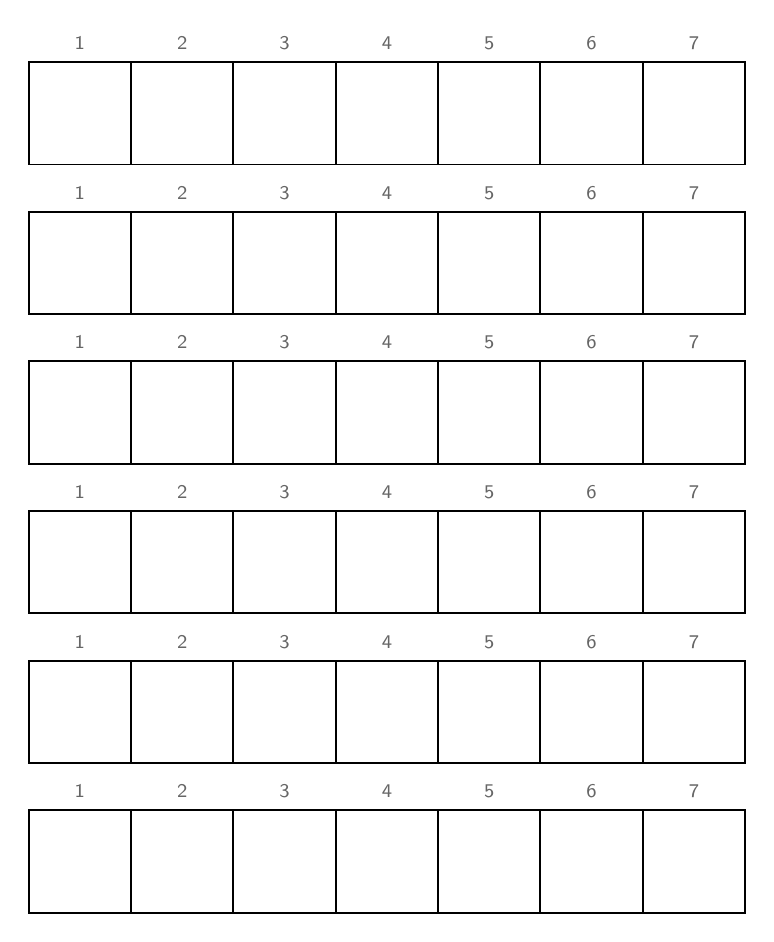
\begin{tikzpicture}[x=1mm,y=1mm,baseline=0]
\draw[line width=0.7pt] (0,0) rectangle (13,-13);
\node[font=\scriptsize, text=black!60] at (6.5,2.4) {1};
\draw[line width=0.7pt] (13,0) rectangle (26,-13);
\node[font=\scriptsize, text=black!60] at (19.5,2.4) {2};
\draw[line width=0.7pt] (26,0) rectangle (39,-13);
\node[font=\scriptsize, text=black!60] at (32.5,2.4) {3};
\draw[line width=0.7pt] (39,0) rectangle (52,-13);
\node[font=\scriptsize, text=black!60] at (45.5,2.4) {4};
\draw[line width=0.7pt] (52,0) rectangle (65,-13);
\node[font=\scriptsize, text=black!60] at (58.5,2.4) {5};
\draw[line width=0.7pt] (65,0) rectangle (78,-13);
\node[font=\scriptsize, text=black!60] at (71.5,2.4) {6};
\draw[line width=0.7pt] (78,0) rectangle (91,-13);
\node[font=\scriptsize, text=black!60] at (84.5,2.4) {7};
\draw[line width=0.7pt] (0,-19) rectangle (13,-32);
\node[font=\scriptsize, text=black!60] at (6.5,-16.6) {1};
\draw[line width=0.7pt] (13,-19) rectangle (26,-32);
\node[font=\scriptsize, text=black!60] at (19.5,-16.6) {2};
\draw[line width=0.7pt] (26,-19) rectangle (39,-32);
\node[font=\scriptsize, text=black!60] at (32.5,-16.6) {3};
\draw[line width=0.7pt] (39,-19) rectangle (52,-32);
\node[font=\scriptsize, text=black!60] at (45.5,-16.6) {4};
\draw[line width=0.7pt] (52,-19) rectangle (65,-32);
\node[font=\scriptsize, text=black!60] at (58.5,-16.6) {5};
\draw[line width=0.7pt] (65,-19) rectangle (78,-32);
\node[font=\scriptsize, text=black!60] at (71.5,-16.6) {6};
\draw[line width=0.7pt] (78,-19) rectangle (91,-32);
\node[font=\scriptsize, text=black!60] at (84.5,-16.6) {7};
\draw[line width=0.7pt] (0,-38) rectangle (13,-51);
\node[font=\scriptsize, text=black!60] at (6.5,-35.6) {1};
\draw[line width=0.7pt] (13,-38) rectangle (26,-51);
\node[font=\scriptsize, text=black!60] at (19.5,-35.6) {2};
\draw[line width=0.7pt] (26,-38) rectangle (39,-51);
\node[font=\scriptsize, text=black!60] at (32.5,-35.6) {3};
\draw[line width=0.7pt] (39,-38) rectangle (52,-51);
\node[font=\scriptsize, text=black!60] at (45.5,-35.6) {4};
\draw[line width=0.7pt] (52,-38) rectangle (65,-51);
\node[font=\scriptsize, text=black!60] at (58.5,-35.6) {5};
\draw[line width=0.7pt] (65,-38) rectangle (78,-51);
\node[font=\scriptsize, text=black!60] at (71.5,-35.6) {6};
\draw[line width=0.7pt] (78,-38) rectangle (91,-51);
\node[font=\scriptsize, text=black!60] at (84.5,-35.6) {7};
\draw[line width=0.7pt] (0,-57) rectangle (13,-70);
\node[font=\scriptsize, text=black!60] at (6.5,-54.6) {1};
\draw[line width=0.7pt] (13,-57) rectangle (26,-70);
\node[font=\scriptsize, text=black!60] at (19.5,-54.6) {2};
\draw[line width=0.7pt] (26,-57) rectangle (39,-70);
\node[font=\scriptsize, text=black!60] at (32.5,-54.6) {3};
\draw[line width=0.7pt] (39,-57) rectangle (52,-70);
\node[font=\scriptsize, text=black!60] at (45.5,-54.6) {4};
\draw[line width=0.7pt] (52,-57) rectangle (65,-70);
\node[font=\scriptsize, text=black!60] at (58.5,-54.6) {5};
\draw[line width=0.7pt] (65,-57) rectangle (78,-70);
\node[font=\scriptsize, text=black!60] at (71.5,-54.6) {6};
\draw[line width=0.7pt] (78,-57) rectangle (91,-70);
\node[font=\scriptsize, text=black!60] at (84.5,-54.6) {7};
\draw[line width=0.7pt] (0,-76) rectangle (13,-89);
\node[font=\scriptsize, text=black!60] at (6.5,-73.6) {1};
\draw[line width=0.7pt] (13,-76) rectangle (26,-89);
\node[font=\scriptsize, text=black!60] at (19.5,-73.6) {2};
\draw[line width=0.7pt] (26,-76) rectangle (39,-89);
\node[font=\scriptsize, text=black!60] at (32.5,-73.6) {3};
\draw[line width=0.7pt] (39,-76) rectangle (52,-89);
\node[font=\scriptsize, text=black!60] at (45.5,-73.6) {4};
\draw[line width=0.7pt] (52,-76) rectangle (65,-89);
\node[font=\scriptsize, text=black!60] at (58.5,-73.6) {5};
\draw[line width=0.7pt] (65,-76) rectangle (78,-89);
\node[font=\scriptsize, text=black!60] at (71.5,-73.6) {6};
\draw[line width=0.7pt] (78,-76) rectangle (91,-89);
\node[font=\scriptsize, text=black!60] at (84.5,-73.6) {7};
\draw[line width=0.7pt] (0,-95) rectangle (13,-108);
\node[font=\scriptsize, text=black!60] at (6.5,-92.6) {1};
\draw[line width=0.7pt] (13,-95) rectangle (26,-108);
\node[font=\scriptsize, text=black!60] at (19.5,-92.6) {2};
\draw[line width=0.7pt] (26,-95) rectangle (39,-108);
\node[font=\scriptsize, text=black!60] at (32.5,-92.6) {3};
\draw[line width=0.7pt] (39,-95) rectangle (52,-108);
\node[font=\scriptsize, text=black!60] at (45.5,-92.6) {4};
\draw[line width=0.7pt] (52,-95) rectangle (65,-108);
\node[font=\scriptsize, text=black!60] at (58.5,-92.6) {5};
\draw[line width=0.7pt] (65,-95) rectangle (78,-108);
\node[font=\scriptsize, text=black!60] at (71.5,-92.6) {6};
\draw[line width=0.7pt] (78,-95) rectangle (91,-108);
\node[font=\scriptsize, text=black!60] at (84.5,-92.6) {7};
\end{tikzpicture}
\end{center}
\vspace{5mm}
\problem{4}{Your partner sets the card and sends one counter. Guess where each counter in the table will land, and then send counters to see. Play again with the coin.}
\vspace{6mm}
\begin{center}
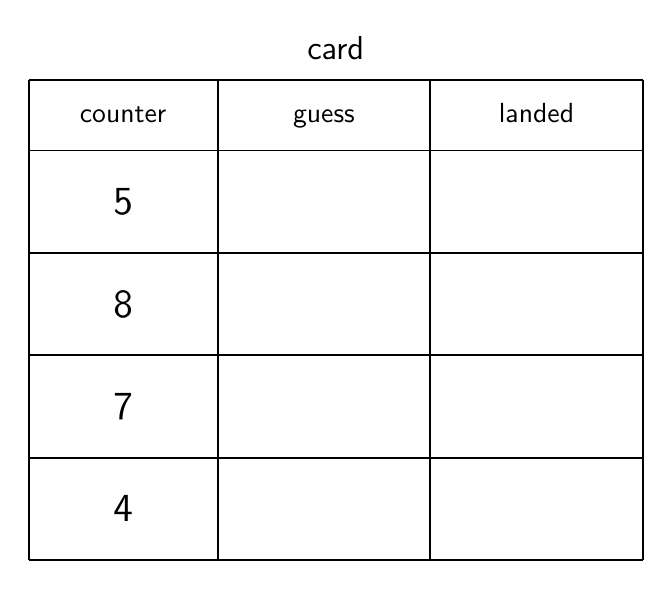
\begin{tikzpicture}[x=1mm,y=1mm,baseline=0]
\node[font=\large, anchor=base] at (39.0,2.5) {card};
\node[font=\normalsize, text height=1.6ex, text depth=0.45ex] at (12.0,-4.5) {counter};
\node[font=\normalsize, text height=1.6ex, text depth=0.45ex] at (37.5,-4.5) {guess};
\node[font=\normalsize, text height=1.6ex, text depth=0.45ex] at (64.5,-4.5) {landed};
\draw[line width=0.7pt] (0,0) -- (0,-61);
\draw[line width=0.7pt] (24,0) -- (24,-61);
\draw[line width=0.7pt] (51,0) -- (51,-61);
\draw[line width=0.7pt] (78,0) -- (78,-61);
\draw[line width=0.7pt] (0,0) -- (78,0);
\draw[line width=0.7pt] (0,-9) -- (78,-9);
\draw[line width=0.7pt] (0,-22) -- (78,-22);
\draw[line width=0.7pt] (0,-35) -- (78,-35);
\draw[line width=0.7pt] (0,-48) -- (78,-48);
\draw[line width=0.7pt] (0,-61) -- (78,-61);
\node[font=\Large] at (12.0,-15.5) {5};
\node[font=\Large] at (12.0,-28.5) {8};
\node[font=\Large] at (12.0,-41.5) {7};
\node[font=\Large] at (12.0,-54.5) {4};
\end{tikzpicture}\hspace{18mm}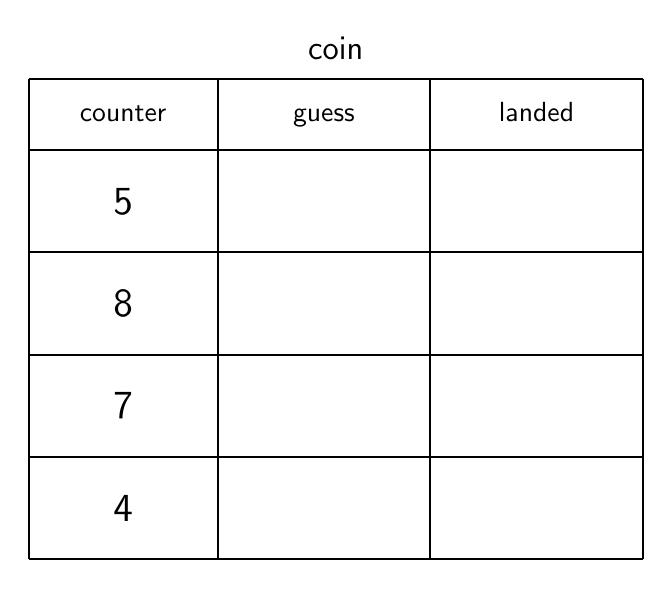
\begin{tikzpicture}[x=1mm,y=1mm,baseline=0]
\node[font=\large, anchor=base] at (39.0,2.5) {coin};
\node[font=\normalsize, text height=1.6ex, text depth=0.45ex] at (12.0,-4.5) {counter};
\node[font=\normalsize, text height=1.6ex, text depth=0.45ex] at (37.5,-4.5) {guess};
\node[font=\normalsize, text height=1.6ex, text depth=0.45ex] at (64.5,-4.5) {landed};
\draw[line width=0.7pt] (0,0) -- (0,-61);
\draw[line width=0.7pt] (24,0) -- (24,-61);
\draw[line width=0.7pt] (51,0) -- (51,-61);
\draw[line width=0.7pt] (78,0) -- (78,-61);
\draw[line width=0.7pt] (0,0) -- (78,0);
\draw[line width=0.7pt] (0,-9) -- (78,-9);
\draw[line width=0.7pt] (0,-22) -- (78,-22);
\draw[line width=0.7pt] (0,-35) -- (78,-35);
\draw[line width=0.7pt] (0,-48) -- (78,-48);
\draw[line width=0.7pt] (0,-61) -- (78,-61);
\node[font=\Large] at (12.0,-15.5) {5};
\node[font=\Large] at (12.0,-28.5) {8};
\node[font=\Large] at (12.0,-41.5) {7};
\node[font=\Large] at (12.0,-54.5) {4};
\end{tikzpicture}
\end{center}
\newpage
\problem{5}{Set the three cards on the board with exits A, B, C and D, draw your starting arrows, and send four counters. Can two of the four counters land on the same exit?}
\vspace{9mm}
\noindent 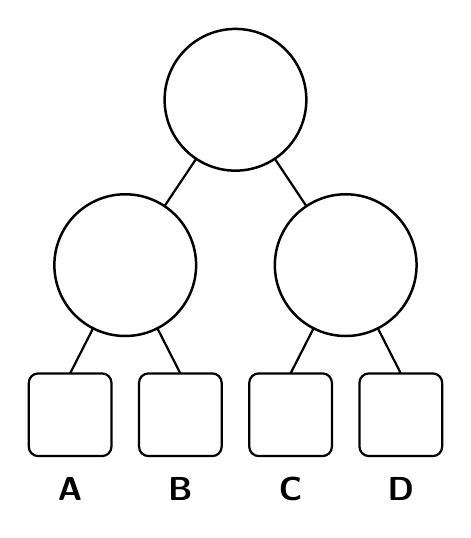
\begin{tikzpicture}[x=1mm,y=1mm,baseline=0]
\draw[line width=0.9pt] (0,0) circle (9.0);
\draw[line width=0.9pt] (-14,-21) circle (9.0);
\draw[line width=0.8pt] (-4.99,-7.49) -- (-9.01,-13.51);
\draw[line width=0.8pt] (-18.08,-29.02) -- (-21.00,-34.75);
\draw[line width=0.8pt, rounded corners=1.2mm] (-26.25,-45.25) rectangle (-15.75,-34.75);
\node[font=\bfseries\large] at (-21.00,-49.45) {A};
\draw[line width=0.8pt] (-9.92,-29.02) -- (-7.00,-34.75);
\draw[line width=0.8pt, rounded corners=1.2mm] (-12.25,-45.25) rectangle (-1.75,-34.75);
\node[font=\bfseries\large] at (-7.00,-49.45) {B};
\draw[line width=0.9pt] (14,-21) circle (9.0);
\draw[line width=0.8pt] (4.99,-7.49) -- (9.01,-13.51);
\draw[line width=0.8pt] (9.92,-29.02) -- (7.00,-34.75);
\draw[line width=0.8pt, rounded corners=1.2mm] (1.75,-45.25) rectangle (12.25,-34.75);
\node[font=\bfseries\large] at (7.00,-49.45) {C};
\draw[line width=0.8pt] (18.08,-29.02) -- (21.00,-34.75);
\draw[line width=0.8pt, rounded corners=1.2mm] (15.75,-45.25) rectangle (26.25,-34.75);
\node[font=\bfseries\large] at (21.00,-49.45) {D};
\end{tikzpicture}\hfill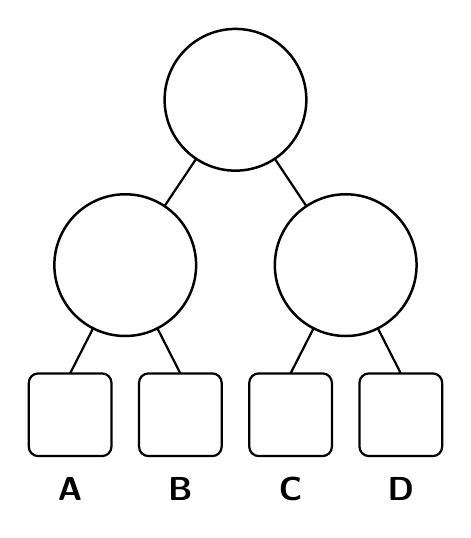
\begin{tikzpicture}[x=1mm,y=1mm,baseline=0]
\draw[line width=0.9pt] (0,0) circle (9.0);
\draw[line width=0.9pt] (-14,-21) circle (9.0);
\draw[line width=0.8pt] (-4.99,-7.49) -- (-9.01,-13.51);
\draw[line width=0.8pt] (-18.08,-29.02) -- (-21.00,-34.75);
\draw[line width=0.8pt, rounded corners=1.2mm] (-26.25,-45.25) rectangle (-15.75,-34.75);
\node[font=\bfseries\large] at (-21.00,-49.45) {A};
\draw[line width=0.8pt] (-9.92,-29.02) -- (-7.00,-34.75);
\draw[line width=0.8pt, rounded corners=1.2mm] (-12.25,-45.25) rectangle (-1.75,-34.75);
\node[font=\bfseries\large] at (-7.00,-49.45) {B};
\draw[line width=0.9pt] (14,-21) circle (9.0);
\draw[line width=0.8pt] (4.99,-7.49) -- (9.01,-13.51);
\draw[line width=0.8pt] (9.92,-29.02) -- (7.00,-34.75);
\draw[line width=0.8pt, rounded corners=1.2mm] (1.75,-45.25) rectangle (12.25,-34.75);
\node[font=\bfseries\large] at (7.00,-49.45) {C};
\draw[line width=0.8pt] (18.08,-29.02) -- (21.00,-34.75);
\draw[line width=0.8pt, rounded corners=1.2mm] (15.75,-45.25) rectangle (26.25,-34.75);
\node[font=\bfseries\large] at (21.00,-49.45) {D};
\end{tikzpicture}\hfill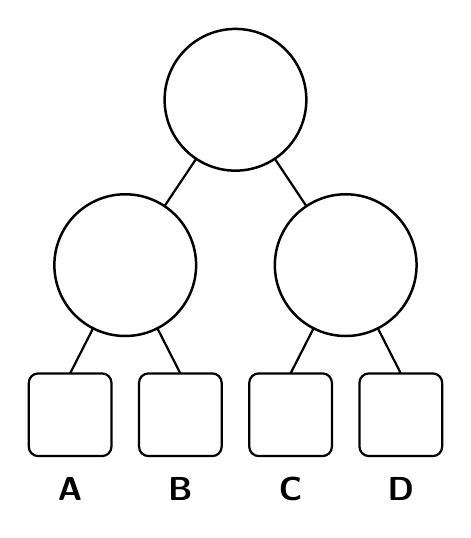
\begin{tikzpicture}[x=1mm,y=1mm,baseline=0]
\draw[line width=0.9pt] (0,0) circle (9.0);
\draw[line width=0.9pt] (-14,-21) circle (9.0);
\draw[line width=0.8pt] (-4.99,-7.49) -- (-9.01,-13.51);
\draw[line width=0.8pt] (-18.08,-29.02) -- (-21.00,-34.75);
\draw[line width=0.8pt, rounded corners=1.2mm] (-26.25,-45.25) rectangle (-15.75,-34.75);
\node[font=\bfseries\large] at (-21.00,-49.45) {A};
\draw[line width=0.8pt] (-9.92,-29.02) -- (-7.00,-34.75);
\draw[line width=0.8pt, rounded corners=1.2mm] (-12.25,-45.25) rectangle (-1.75,-34.75);
\node[font=\bfseries\large] at (-7.00,-49.45) {B};
\draw[line width=0.9pt] (14,-21) circle (9.0);
\draw[line width=0.8pt] (4.99,-7.49) -- (9.01,-13.51);
\draw[line width=0.8pt] (9.92,-29.02) -- (7.00,-34.75);
\draw[line width=0.8pt, rounded corners=1.2mm] (1.75,-45.25) rectangle (12.25,-34.75);
\node[font=\bfseries\large] at (7.00,-49.45) {C};
\draw[line width=0.8pt] (18.08,-29.02) -- (21.00,-34.75);
\draw[line width=0.8pt, rounded corners=1.2mm] (15.75,-45.25) rectangle (26.25,-34.75);
\node[font=\bfseries\large] at (21.00,-49.45) {D};
\end{tikzpicture}

\vspace{7mm}
\noindent 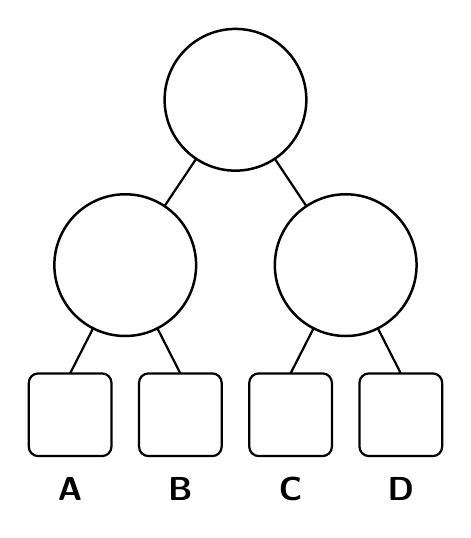
\begin{tikzpicture}[x=1mm,y=1mm,baseline=0]
\draw[line width=0.9pt] (0,0) circle (9.0);
\draw[line width=0.9pt] (-14,-21) circle (9.0);
\draw[line width=0.8pt] (-4.99,-7.49) -- (-9.01,-13.51);
\draw[line width=0.8pt] (-18.08,-29.02) -- (-21.00,-34.75);
\draw[line width=0.8pt, rounded corners=1.2mm] (-26.25,-45.25) rectangle (-15.75,-34.75);
\node[font=\bfseries\large] at (-21.00,-49.45) {A};
\draw[line width=0.8pt] (-9.92,-29.02) -- (-7.00,-34.75);
\draw[line width=0.8pt, rounded corners=1.2mm] (-12.25,-45.25) rectangle (-1.75,-34.75);
\node[font=\bfseries\large] at (-7.00,-49.45) {B};
\draw[line width=0.9pt] (14,-21) circle (9.0);
\draw[line width=0.8pt] (4.99,-7.49) -- (9.01,-13.51);
\draw[line width=0.8pt] (9.92,-29.02) -- (7.00,-34.75);
\draw[line width=0.8pt, rounded corners=1.2mm] (1.75,-45.25) rectangle (12.25,-34.75);
\node[font=\bfseries\large] at (7.00,-49.45) {C};
\draw[line width=0.8pt] (18.08,-29.02) -- (21.00,-34.75);
\draw[line width=0.8pt, rounded corners=1.2mm] (15.75,-45.25) rectangle (26.25,-34.75);
\node[font=\bfseries\large] at (21.00,-49.45) {D};
\end{tikzpicture}\hfill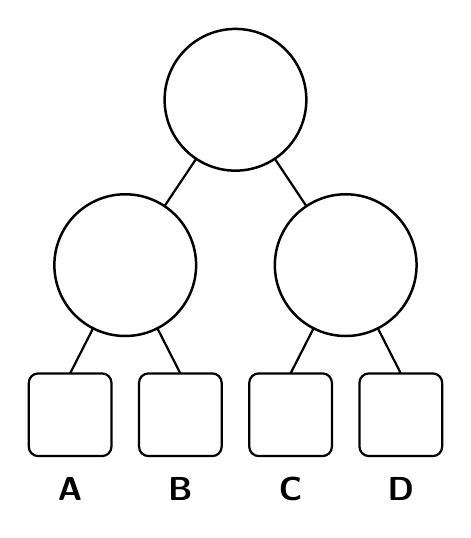
\begin{tikzpicture}[x=1mm,y=1mm,baseline=0]
\draw[line width=0.9pt] (0,0) circle (9.0);
\draw[line width=0.9pt] (-14,-21) circle (9.0);
\draw[line width=0.8pt] (-4.99,-7.49) -- (-9.01,-13.51);
\draw[line width=0.8pt] (-18.08,-29.02) -- (-21.00,-34.75);
\draw[line width=0.8pt, rounded corners=1.2mm] (-26.25,-45.25) rectangle (-15.75,-34.75);
\node[font=\bfseries\large] at (-21.00,-49.45) {A};
\draw[line width=0.8pt] (-9.92,-29.02) -- (-7.00,-34.75);
\draw[line width=0.8pt, rounded corners=1.2mm] (-12.25,-45.25) rectangle (-1.75,-34.75);
\node[font=\bfseries\large] at (-7.00,-49.45) {B};
\draw[line width=0.9pt] (14,-21) circle (9.0);
\draw[line width=0.8pt] (4.99,-7.49) -- (9.01,-13.51);
\draw[line width=0.8pt] (9.92,-29.02) -- (7.00,-34.75);
\draw[line width=0.8pt, rounded corners=1.2mm] (1.75,-45.25) rectangle (12.25,-34.75);
\node[font=\bfseries\large] at (7.00,-49.45) {C};
\draw[line width=0.8pt] (18.08,-29.02) -- (21.00,-34.75);
\draw[line width=0.8pt, rounded corners=1.2mm] (15.75,-45.25) rectangle (26.25,-34.75);
\node[font=\bfseries\large] at (21.00,-49.45) {D};
\end{tikzpicture}\hfill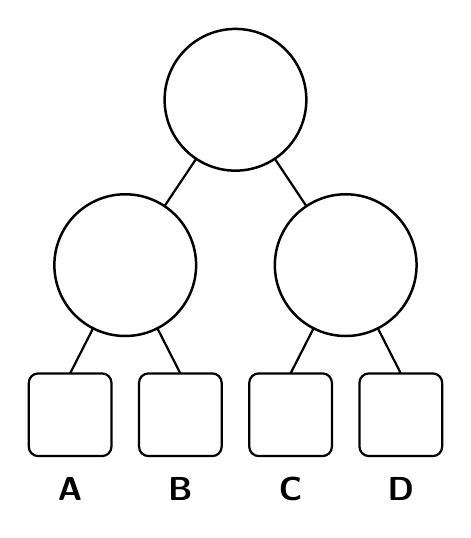
\begin{tikzpicture}[x=1mm,y=1mm,baseline=0]
\draw[line width=0.9pt] (0,0) circle (9.0);
\draw[line width=0.9pt] (-14,-21) circle (9.0);
\draw[line width=0.8pt] (-4.99,-7.49) -- (-9.01,-13.51);
\draw[line width=0.8pt] (-18.08,-29.02) -- (-21.00,-34.75);
\draw[line width=0.8pt, rounded corners=1.2mm] (-26.25,-45.25) rectangle (-15.75,-34.75);
\node[font=\bfseries\large] at (-21.00,-49.45) {A};
\draw[line width=0.8pt] (-9.92,-29.02) -- (-7.00,-34.75);
\draw[line width=0.8pt, rounded corners=1.2mm] (-12.25,-45.25) rectangle (-1.75,-34.75);
\node[font=\bfseries\large] at (-7.00,-49.45) {B};
\draw[line width=0.9pt] (14,-21) circle (9.0);
\draw[line width=0.8pt] (4.99,-7.49) -- (9.01,-13.51);
\draw[line width=0.8pt] (9.92,-29.02) -- (7.00,-34.75);
\draw[line width=0.8pt, rounded corners=1.2mm] (1.75,-45.25) rectangle (12.25,-34.75);
\node[font=\bfseries\large] at (7.00,-49.45) {C};
\draw[line width=0.8pt] (18.08,-29.02) -- (21.00,-34.75);
\draw[line width=0.8pt, rounded corners=1.2mm] (15.75,-45.25) rectangle (26.25,-34.75);
\node[font=\bfseries\large] at (21.00,-49.45) {D};
\end{tikzpicture}

\vspace{7mm}
\noindent 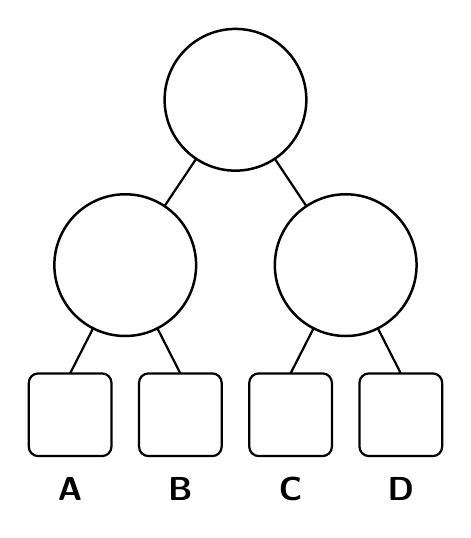
\begin{tikzpicture}[x=1mm,y=1mm,baseline=0]
\draw[line width=0.9pt] (0,0) circle (9.0);
\draw[line width=0.9pt] (-14,-21) circle (9.0);
\draw[line width=0.8pt] (-4.99,-7.49) -- (-9.01,-13.51);
\draw[line width=0.8pt] (-18.08,-29.02) -- (-21.00,-34.75);
\draw[line width=0.8pt, rounded corners=1.2mm] (-26.25,-45.25) rectangle (-15.75,-34.75);
\node[font=\bfseries\large] at (-21.00,-49.45) {A};
\draw[line width=0.8pt] (-9.92,-29.02) -- (-7.00,-34.75);
\draw[line width=0.8pt, rounded corners=1.2mm] (-12.25,-45.25) rectangle (-1.75,-34.75);
\node[font=\bfseries\large] at (-7.00,-49.45) {B};
\draw[line width=0.9pt] (14,-21) circle (9.0);
\draw[line width=0.8pt] (4.99,-7.49) -- (9.01,-13.51);
\draw[line width=0.8pt] (9.92,-29.02) -- (7.00,-34.75);
\draw[line width=0.8pt, rounded corners=1.2mm] (1.75,-45.25) rectangle (12.25,-34.75);
\node[font=\bfseries\large] at (7.00,-49.45) {C};
\draw[line width=0.8pt] (18.08,-29.02) -- (21.00,-34.75);
\draw[line width=0.8pt, rounded corners=1.2mm] (15.75,-45.25) rectangle (26.25,-34.75);
\node[font=\bfseries\large] at (21.00,-49.45) {D};
\end{tikzpicture}\hfill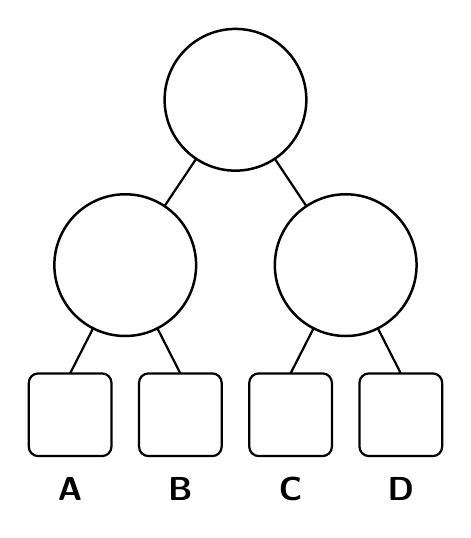
\begin{tikzpicture}[x=1mm,y=1mm,baseline=0]
\draw[line width=0.9pt] (0,0) circle (9.0);
\draw[line width=0.9pt] (-14,-21) circle (9.0);
\draw[line width=0.8pt] (-4.99,-7.49) -- (-9.01,-13.51);
\draw[line width=0.8pt] (-18.08,-29.02) -- (-21.00,-34.75);
\draw[line width=0.8pt, rounded corners=1.2mm] (-26.25,-45.25) rectangle (-15.75,-34.75);
\node[font=\bfseries\large] at (-21.00,-49.45) {A};
\draw[line width=0.8pt] (-9.92,-29.02) -- (-7.00,-34.75);
\draw[line width=0.8pt, rounded corners=1.2mm] (-12.25,-45.25) rectangle (-1.75,-34.75);
\node[font=\bfseries\large] at (-7.00,-49.45) {B};
\draw[line width=0.9pt] (14,-21) circle (9.0);
\draw[line width=0.8pt] (4.99,-7.49) -- (9.01,-13.51);
\draw[line width=0.8pt] (9.92,-29.02) -- (7.00,-34.75);
\draw[line width=0.8pt, rounded corners=1.2mm] (1.75,-45.25) rectangle (12.25,-34.75);
\node[font=\bfseries\large] at (7.00,-49.45) {C};
\draw[line width=0.8pt] (18.08,-29.02) -- (21.00,-34.75);
\draw[line width=0.8pt, rounded corners=1.2mm] (15.75,-45.25) rectangle (26.25,-34.75);
\node[font=\bfseries\large] at (21.00,-49.45) {D};
\end{tikzpicture}\hfill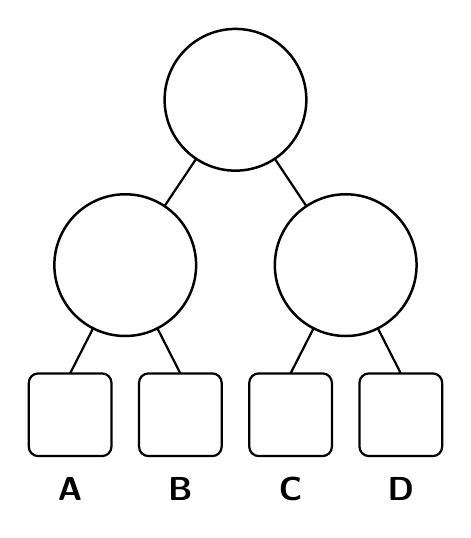
\begin{tikzpicture}[x=1mm,y=1mm,baseline=0]
\draw[line width=0.9pt] (0,0) circle (9.0);
\draw[line width=0.9pt] (-14,-21) circle (9.0);
\draw[line width=0.8pt] (-4.99,-7.49) -- (-9.01,-13.51);
\draw[line width=0.8pt] (-18.08,-29.02) -- (-21.00,-34.75);
\draw[line width=0.8pt, rounded corners=1.2mm] (-26.25,-45.25) rectangle (-15.75,-34.75);
\node[font=\bfseries\large] at (-21.00,-49.45) {A};
\draw[line width=0.8pt] (-9.92,-29.02) -- (-7.00,-34.75);
\draw[line width=0.8pt, rounded corners=1.2mm] (-12.25,-45.25) rectangle (-1.75,-34.75);
\node[font=\bfseries\large] at (-7.00,-49.45) {B};
\draw[line width=0.9pt] (14,-21) circle (9.0);
\draw[line width=0.8pt] (4.99,-7.49) -- (9.01,-13.51);
\draw[line width=0.8pt] (9.92,-29.02) -- (7.00,-34.75);
\draw[line width=0.8pt, rounded corners=1.2mm] (1.75,-45.25) rectangle (12.25,-34.75);
\node[font=\bfseries\large] at (7.00,-49.45) {C};
\draw[line width=0.8pt] (18.08,-29.02) -- (21.00,-34.75);
\draw[line width=0.8pt, rounded corners=1.2mm] (15.75,-45.25) rectangle (26.25,-34.75);
\node[font=\bfseries\large] at (21.00,-49.45) {D};
\end{tikzpicture}

\newpage
\problem{6}{Send counters on the A, B, C, D board to make the piles in each picture, and draw the starting arrows that make them. Cross out any picture that no starting arrows can make.}
\vspace{12mm}
\noindent\hfill 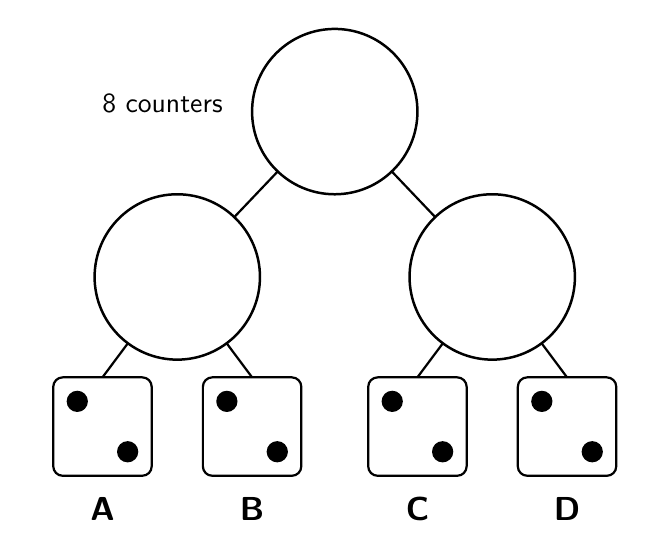
\begin{tikzpicture}[x=1mm,y=1mm,baseline=0]
\draw[line width=0.9pt] (0,0) circle (10.5);
\draw[line width=0.9pt] (-20,-21) circle (10.5);
\draw[line width=0.8pt] (-7.24,-7.60) -- (-12.76,-13.40);
\draw[line width=0.8pt] (-26.27,-29.42) -- (-29.50,-33.75);
\draw[line width=0.8pt, rounded corners=1.2mm] (-35.75,-46.25) rectangle (-23.25,-33.75);
\node[font=\bfseries\large] at (-29.50,-50.45) {A};
\fill (-32.70,-36.80) circle (1.35);\fill (-26.30,-43.20) circle (1.35);
\draw[line width=0.8pt] (-13.73,-29.42) -- (-10.50,-33.75);
\draw[line width=0.8pt, rounded corners=1.2mm] (-16.75,-46.25) rectangle (-4.25,-33.75);
\node[font=\bfseries\large] at (-10.50,-50.45) {B};
\fill (-13.70,-36.80) circle (1.35);\fill (-7.30,-43.20) circle (1.35);
\draw[line width=0.9pt] (20,-21) circle (10.5);
\draw[line width=0.8pt] (7.24,-7.60) -- (12.76,-13.40);
\draw[line width=0.8pt] (13.73,-29.42) -- (10.50,-33.75);
\draw[line width=0.8pt, rounded corners=1.2mm] (4.25,-46.25) rectangle (16.75,-33.75);
\node[font=\bfseries\large] at (10.50,-50.45) {C};
\fill (7.30,-36.80) circle (1.35);\fill (13.70,-43.20) circle (1.35);
\draw[line width=0.8pt] (26.27,-29.42) -- (29.50,-33.75);
\draw[line width=0.8pt, rounded corners=1.2mm] (23.25,-46.25) rectangle (35.75,-33.75);
\node[font=\bfseries\large] at (29.50,-50.45) {D};
\fill (26.30,-36.80) circle (1.35);\fill (32.70,-43.20) circle (1.35);
\node[font=\normalsize, anchor=east] at (-13.00,1) {8 counters};
\path (-39,0) (39,0);
\end{tikzpicture}\hspace{22mm}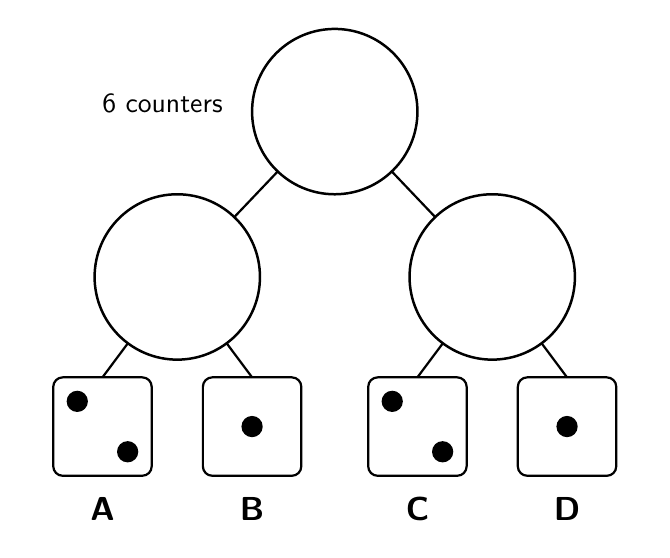
\begin{tikzpicture}[x=1mm,y=1mm,baseline=0]
\draw[line width=0.9pt] (0,0) circle (10.5);
\draw[line width=0.9pt] (-20,-21) circle (10.5);
\draw[line width=0.8pt] (-7.24,-7.60) -- (-12.76,-13.40);
\draw[line width=0.8pt] (-26.27,-29.42) -- (-29.50,-33.75);
\draw[line width=0.8pt, rounded corners=1.2mm] (-35.75,-46.25) rectangle (-23.25,-33.75);
\node[font=\bfseries\large] at (-29.50,-50.45) {A};
\fill (-32.70,-36.80) circle (1.35);\fill (-26.30,-43.20) circle (1.35);
\draw[line width=0.8pt] (-13.73,-29.42) -- (-10.50,-33.75);
\draw[line width=0.8pt, rounded corners=1.2mm] (-16.75,-46.25) rectangle (-4.25,-33.75);
\node[font=\bfseries\large] at (-10.50,-50.45) {B};
\fill (-10.50,-40.00) circle (1.35);
\draw[line width=0.9pt] (20,-21) circle (10.5);
\draw[line width=0.8pt] (7.24,-7.60) -- (12.76,-13.40);
\draw[line width=0.8pt] (13.73,-29.42) -- (10.50,-33.75);
\draw[line width=0.8pt, rounded corners=1.2mm] (4.25,-46.25) rectangle (16.75,-33.75);
\node[font=\bfseries\large] at (10.50,-50.45) {C};
\fill (7.30,-36.80) circle (1.35);\fill (13.70,-43.20) circle (1.35);
\draw[line width=0.8pt] (26.27,-29.42) -- (29.50,-33.75);
\draw[line width=0.8pt, rounded corners=1.2mm] (23.25,-46.25) rectangle (35.75,-33.75);
\node[font=\bfseries\large] at (29.50,-50.45) {D};
\fill (29.50,-40.00) circle (1.35);
\node[font=\normalsize, anchor=east] at (-13.00,1) {6 counters};
\path (-39,0) (39,0);
\end{tikzpicture}\hfill\null

\vspace{9mm}
\noindent\hfill 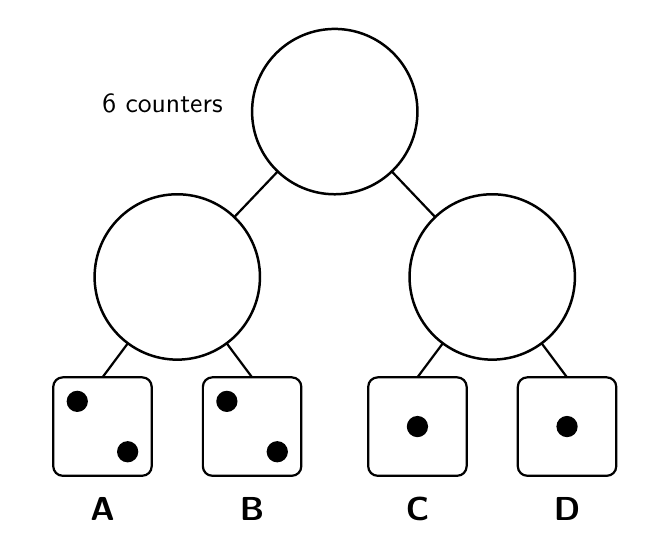
\begin{tikzpicture}[x=1mm,y=1mm,baseline=0]
\draw[line width=0.9pt] (0,0) circle (10.5);
\draw[line width=0.9pt] (-20,-21) circle (10.5);
\draw[line width=0.8pt] (-7.24,-7.60) -- (-12.76,-13.40);
\draw[line width=0.8pt] (-26.27,-29.42) -- (-29.50,-33.75);
\draw[line width=0.8pt, rounded corners=1.2mm] (-35.75,-46.25) rectangle (-23.25,-33.75);
\node[font=\bfseries\large] at (-29.50,-50.45) {A};
\fill (-32.70,-36.80) circle (1.35);\fill (-26.30,-43.20) circle (1.35);
\draw[line width=0.8pt] (-13.73,-29.42) -- (-10.50,-33.75);
\draw[line width=0.8pt, rounded corners=1.2mm] (-16.75,-46.25) rectangle (-4.25,-33.75);
\node[font=\bfseries\large] at (-10.50,-50.45) {B};
\fill (-13.70,-36.80) circle (1.35);\fill (-7.30,-43.20) circle (1.35);
\draw[line width=0.9pt] (20,-21) circle (10.5);
\draw[line width=0.8pt] (7.24,-7.60) -- (12.76,-13.40);
\draw[line width=0.8pt] (13.73,-29.42) -- (10.50,-33.75);
\draw[line width=0.8pt, rounded corners=1.2mm] (4.25,-46.25) rectangle (16.75,-33.75);
\node[font=\bfseries\large] at (10.50,-50.45) {C};
\fill (10.50,-40.00) circle (1.35);
\draw[line width=0.8pt] (26.27,-29.42) -- (29.50,-33.75);
\draw[line width=0.8pt, rounded corners=1.2mm] (23.25,-46.25) rectangle (35.75,-33.75);
\node[font=\bfseries\large] at (29.50,-50.45) {D};
\fill (29.50,-40.00) circle (1.35);
\node[font=\normalsize, anchor=east] at (-13.00,1) {6 counters};
\path (-39,0) (39,0);
\end{tikzpicture}\hspace{22mm}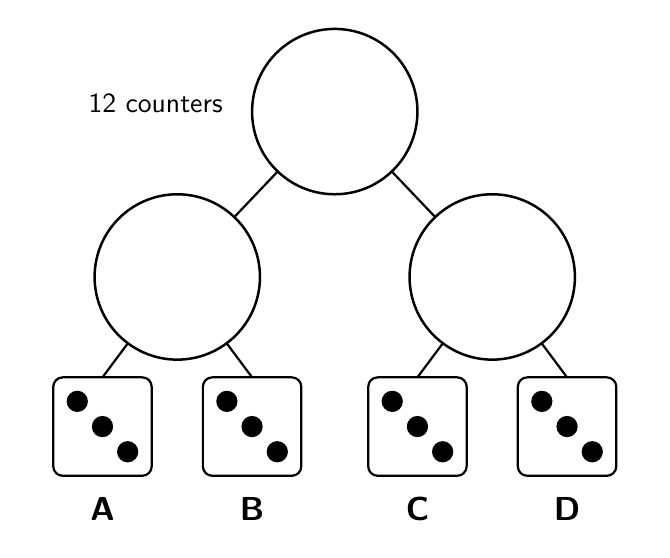
\begin{tikzpicture}[x=1mm,y=1mm,baseline=0]
\draw[line width=0.9pt] (0,0) circle (10.5);
\draw[line width=0.9pt] (-20,-21) circle (10.5);
\draw[line width=0.8pt] (-7.24,-7.60) -- (-12.76,-13.40);
\draw[line width=0.8pt] (-26.27,-29.42) -- (-29.50,-33.75);
\draw[line width=0.8pt, rounded corners=1.2mm] (-35.75,-46.25) rectangle (-23.25,-33.75);
\node[font=\bfseries\large] at (-29.50,-50.45) {A};
\fill (-32.70,-36.80) circle (1.35);\fill (-29.50,-40.00) circle (1.35);\fill (-26.30,-43.20) circle (1.35);
\draw[line width=0.8pt] (-13.73,-29.42) -- (-10.50,-33.75);
\draw[line width=0.8pt, rounded corners=1.2mm] (-16.75,-46.25) rectangle (-4.25,-33.75);
\node[font=\bfseries\large] at (-10.50,-50.45) {B};
\fill (-13.70,-36.80) circle (1.35);\fill (-10.50,-40.00) circle (1.35);\fill (-7.30,-43.20) circle (1.35);
\draw[line width=0.9pt] (20,-21) circle (10.5);
\draw[line width=0.8pt] (7.24,-7.60) -- (12.76,-13.40);
\draw[line width=0.8pt] (13.73,-29.42) -- (10.50,-33.75);
\draw[line width=0.8pt, rounded corners=1.2mm] (4.25,-46.25) rectangle (16.75,-33.75);
\node[font=\bfseries\large] at (10.50,-50.45) {C};
\fill (7.30,-36.80) circle (1.35);\fill (10.50,-40.00) circle (1.35);\fill (13.70,-43.20) circle (1.35);
\draw[line width=0.8pt] (26.27,-29.42) -- (29.50,-33.75);
\draw[line width=0.8pt, rounded corners=1.2mm] (23.25,-46.25) rectangle (35.75,-33.75);
\node[font=\bfseries\large] at (29.50,-50.45) {D};
\fill (26.30,-36.80) circle (1.35);\fill (29.50,-40.00) circle (1.35);\fill (32.70,-43.20) circle (1.35);
\node[font=\normalsize, anchor=east] at (-13.00,1) {12 counters};
\path (-39,0) (39,0);
\end{tikzpicture}\hfill\null

\vspace{9mm}
\noindent\hfill 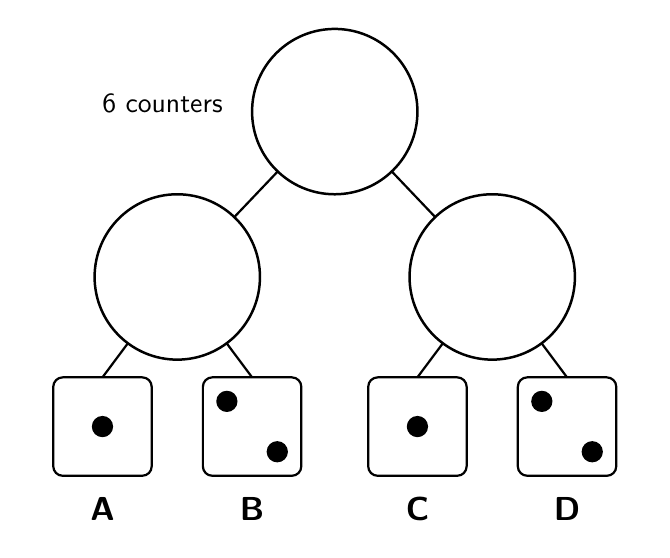
\begin{tikzpicture}[x=1mm,y=1mm,baseline=0]
\draw[line width=0.9pt] (0,0) circle (10.5);
\draw[line width=0.9pt] (-20,-21) circle (10.5);
\draw[line width=0.8pt] (-7.24,-7.60) -- (-12.76,-13.40);
\draw[line width=0.8pt] (-26.27,-29.42) -- (-29.50,-33.75);
\draw[line width=0.8pt, rounded corners=1.2mm] (-35.75,-46.25) rectangle (-23.25,-33.75);
\node[font=\bfseries\large] at (-29.50,-50.45) {A};
\fill (-29.50,-40.00) circle (1.35);
\draw[line width=0.8pt] (-13.73,-29.42) -- (-10.50,-33.75);
\draw[line width=0.8pt, rounded corners=1.2mm] (-16.75,-46.25) rectangle (-4.25,-33.75);
\node[font=\bfseries\large] at (-10.50,-50.45) {B};
\fill (-13.70,-36.80) circle (1.35);\fill (-7.30,-43.20) circle (1.35);
\draw[line width=0.9pt] (20,-21) circle (10.5);
\draw[line width=0.8pt] (7.24,-7.60) -- (12.76,-13.40);
\draw[line width=0.8pt] (13.73,-29.42) -- (10.50,-33.75);
\draw[line width=0.8pt, rounded corners=1.2mm] (4.25,-46.25) rectangle (16.75,-33.75);
\node[font=\bfseries\large] at (10.50,-50.45) {C};
\fill (10.50,-40.00) circle (1.35);
\draw[line width=0.8pt] (26.27,-29.42) -- (29.50,-33.75);
\draw[line width=0.8pt, rounded corners=1.2mm] (23.25,-46.25) rectangle (35.75,-33.75);
\node[font=\bfseries\large] at (29.50,-50.45) {D};
\fill (26.30,-36.80) circle (1.35);\fill (32.70,-43.20) circle (1.35);
\node[font=\normalsize, anchor=east] at (-13.00,1) {6 counters};
\path (-39,0) (39,0);
\end{tikzpicture}\hspace{22mm}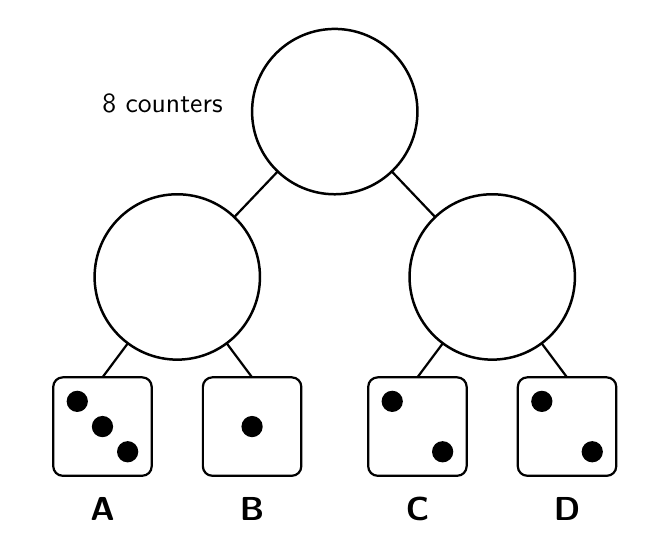
\begin{tikzpicture}[x=1mm,y=1mm,baseline=0]
\draw[line width=0.9pt] (0,0) circle (10.5);
\draw[line width=0.9pt] (-20,-21) circle (10.5);
\draw[line width=0.8pt] (-7.24,-7.60) -- (-12.76,-13.40);
\draw[line width=0.8pt] (-26.27,-29.42) -- (-29.50,-33.75);
\draw[line width=0.8pt, rounded corners=1.2mm] (-35.75,-46.25) rectangle (-23.25,-33.75);
\node[font=\bfseries\large] at (-29.50,-50.45) {A};
\fill (-32.70,-36.80) circle (1.35);\fill (-29.50,-40.00) circle (1.35);\fill (-26.30,-43.20) circle (1.35);
\draw[line width=0.8pt] (-13.73,-29.42) -- (-10.50,-33.75);
\draw[line width=0.8pt, rounded corners=1.2mm] (-16.75,-46.25) rectangle (-4.25,-33.75);
\node[font=\bfseries\large] at (-10.50,-50.45) {B};
\fill (-10.50,-40.00) circle (1.35);
\draw[line width=0.9pt] (20,-21) circle (10.5);
\draw[line width=0.8pt] (7.24,-7.60) -- (12.76,-13.40);
\draw[line width=0.8pt] (13.73,-29.42) -- (10.50,-33.75);
\draw[line width=0.8pt, rounded corners=1.2mm] (4.25,-46.25) rectangle (16.75,-33.75);
\node[font=\bfseries\large] at (10.50,-50.45) {C};
\fill (7.30,-36.80) circle (1.35);\fill (13.70,-43.20) circle (1.35);
\draw[line width=0.8pt] (26.27,-29.42) -- (29.50,-33.75);
\draw[line width=0.8pt, rounded corners=1.2mm] (23.25,-46.25) rectangle (35.75,-33.75);
\node[font=\bfseries\large] at (29.50,-50.45) {D};
\fill (26.30,-36.80) circle (1.35);\fill (32.70,-43.20) circle (1.35);
\node[font=\normalsize, anchor=east] at (-13.00,1) {8 counters};
\path (-39,0) (39,0);
\end{tikzpicture}\hfill\null

\newpage
\problem{7}{Draw starting arrows that make B the first exit to get two counters. Then draw starting arrows that make B the last exit to get two counters.}
\vspace{10mm}
\noindent\hfill 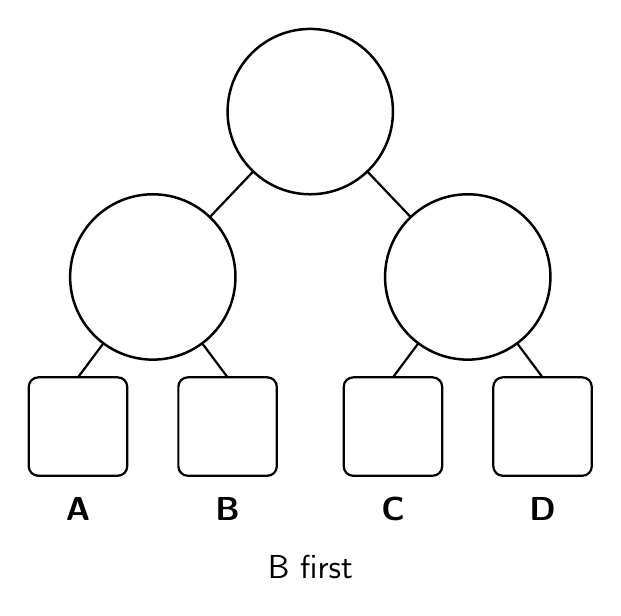
\begin{tikzpicture}[x=1mm,y=1mm,baseline=0]
\draw[line width=0.9pt] (0,0) circle (10.5);
\draw[line width=0.9pt] (-20,-21) circle (10.5);
\draw[line width=0.8pt] (-7.24,-7.60) -- (-12.76,-13.40);
\draw[line width=0.8pt] (-26.27,-29.42) -- (-29.50,-33.75);
\draw[line width=0.8pt, rounded corners=1.2mm] (-35.75,-46.25) rectangle (-23.25,-33.75);
\node[font=\bfseries\large] at (-29.50,-50.45) {A};
\draw[line width=0.8pt] (-13.73,-29.42) -- (-10.50,-33.75);
\draw[line width=0.8pt, rounded corners=1.2mm] (-16.75,-46.25) rectangle (-4.25,-33.75);
\node[font=\bfseries\large] at (-10.50,-50.45) {B};
\draw[line width=0.9pt] (20,-21) circle (10.5);
\draw[line width=0.8pt] (7.24,-7.60) -- (12.76,-13.40);
\draw[line width=0.8pt] (13.73,-29.42) -- (10.50,-33.75);
\draw[line width=0.8pt, rounded corners=1.2mm] (4.25,-46.25) rectangle (16.75,-33.75);
\node[font=\bfseries\large] at (10.50,-50.45) {C};
\draw[line width=0.8pt] (26.27,-29.42) -- (29.50,-33.75);
\draw[line width=0.8pt, rounded corners=1.2mm] (23.25,-46.25) rectangle (35.75,-33.75);
\node[font=\bfseries\large] at (29.50,-50.45) {D};
\node[font=\large, anchor=base] at (0,-59.25) {B first};
\end{tikzpicture}\hspace{24mm}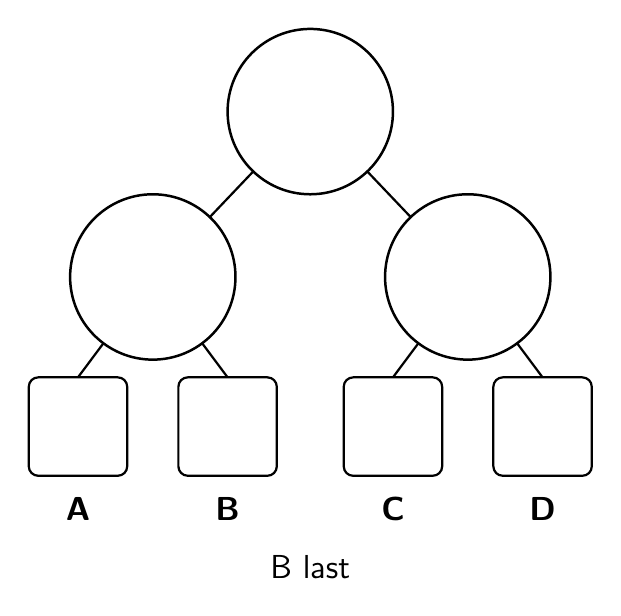
\begin{tikzpicture}[x=1mm,y=1mm,baseline=0]
\draw[line width=0.9pt] (0,0) circle (10.5);
\draw[line width=0.9pt] (-20,-21) circle (10.5);
\draw[line width=0.8pt] (-7.24,-7.60) -- (-12.76,-13.40);
\draw[line width=0.8pt] (-26.27,-29.42) -- (-29.50,-33.75);
\draw[line width=0.8pt, rounded corners=1.2mm] (-35.75,-46.25) rectangle (-23.25,-33.75);
\node[font=\bfseries\large] at (-29.50,-50.45) {A};
\draw[line width=0.8pt] (-13.73,-29.42) -- (-10.50,-33.75);
\draw[line width=0.8pt, rounded corners=1.2mm] (-16.75,-46.25) rectangle (-4.25,-33.75);
\node[font=\bfseries\large] at (-10.50,-50.45) {B};
\draw[line width=0.9pt] (20,-21) circle (10.5);
\draw[line width=0.8pt] (7.24,-7.60) -- (12.76,-13.40);
\draw[line width=0.8pt] (13.73,-29.42) -- (10.50,-33.75);
\draw[line width=0.8pt, rounded corners=1.2mm] (4.25,-46.25) rectangle (16.75,-33.75);
\node[font=\bfseries\large] at (10.50,-50.45) {C};
\draw[line width=0.8pt] (26.27,-29.42) -- (29.50,-33.75);
\draw[line width=0.8pt, rounded corners=1.2mm] (23.25,-46.25) rectangle (35.75,-33.75);
\node[font=\bfseries\large] at (29.50,-50.45) {D};
\node[font=\large, anchor=base] at (0,-59.25) {B last};
\end{tikzpicture}\hfill\null

\vspace{12mm}
\problem{8}{Draw every way to set the three cards so that the first counter lands on C.}
\vspace{10mm}
\noindent 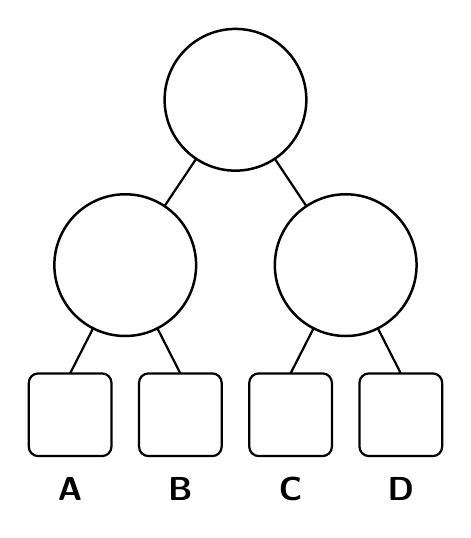
\begin{tikzpicture}[x=1mm,y=1mm,baseline=0]
\draw[line width=0.9pt] (0,0) circle (9.0);
\draw[line width=0.9pt] (-14,-21) circle (9.0);
\draw[line width=0.8pt] (-4.99,-7.49) -- (-9.01,-13.51);
\draw[line width=0.8pt] (-18.08,-29.02) -- (-21.00,-34.75);
\draw[line width=0.8pt, rounded corners=1.2mm] (-26.25,-45.25) rectangle (-15.75,-34.75);
\node[font=\bfseries\large] at (-21.00,-49.45) {A};
\draw[line width=0.8pt] (-9.92,-29.02) -- (-7.00,-34.75);
\draw[line width=0.8pt, rounded corners=1.2mm] (-12.25,-45.25) rectangle (-1.75,-34.75);
\node[font=\bfseries\large] at (-7.00,-49.45) {B};
\draw[line width=0.9pt] (14,-21) circle (9.0);
\draw[line width=0.8pt] (4.99,-7.49) -- (9.01,-13.51);
\draw[line width=0.8pt] (9.92,-29.02) -- (7.00,-34.75);
\draw[line width=0.8pt, rounded corners=1.2mm] (1.75,-45.25) rectangle (12.25,-34.75);
\node[font=\bfseries\large] at (7.00,-49.45) {C};
\draw[line width=0.8pt] (18.08,-29.02) -- (21.00,-34.75);
\draw[line width=0.8pt, rounded corners=1.2mm] (15.75,-45.25) rectangle (26.25,-34.75);
\node[font=\bfseries\large] at (21.00,-49.45) {D};
\end{tikzpicture}\hfill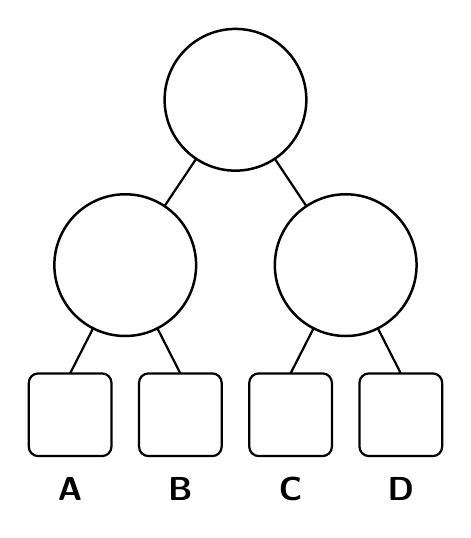
\begin{tikzpicture}[x=1mm,y=1mm,baseline=0]
\draw[line width=0.9pt] (0,0) circle (9.0);
\draw[line width=0.9pt] (-14,-21) circle (9.0);
\draw[line width=0.8pt] (-4.99,-7.49) -- (-9.01,-13.51);
\draw[line width=0.8pt] (-18.08,-29.02) -- (-21.00,-34.75);
\draw[line width=0.8pt, rounded corners=1.2mm] (-26.25,-45.25) rectangle (-15.75,-34.75);
\node[font=\bfseries\large] at (-21.00,-49.45) {A};
\draw[line width=0.8pt] (-9.92,-29.02) -- (-7.00,-34.75);
\draw[line width=0.8pt, rounded corners=1.2mm] (-12.25,-45.25) rectangle (-1.75,-34.75);
\node[font=\bfseries\large] at (-7.00,-49.45) {B};
\draw[line width=0.9pt] (14,-21) circle (9.0);
\draw[line width=0.8pt] (4.99,-7.49) -- (9.01,-13.51);
\draw[line width=0.8pt] (9.92,-29.02) -- (7.00,-34.75);
\draw[line width=0.8pt, rounded corners=1.2mm] (1.75,-45.25) rectangle (12.25,-34.75);
\node[font=\bfseries\large] at (7.00,-49.45) {C};
\draw[line width=0.8pt] (18.08,-29.02) -- (21.00,-34.75);
\draw[line width=0.8pt, rounded corners=1.2mm] (15.75,-45.25) rectangle (26.25,-34.75);
\node[font=\bfseries\large] at (21.00,-49.45) {D};
\end{tikzpicture}\hfill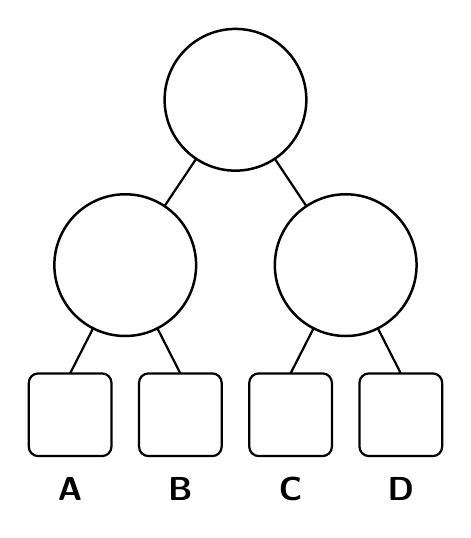
\begin{tikzpicture}[x=1mm,y=1mm,baseline=0]
\draw[line width=0.9pt] (0,0) circle (9.0);
\draw[line width=0.9pt] (-14,-21) circle (9.0);
\draw[line width=0.8pt] (-4.99,-7.49) -- (-9.01,-13.51);
\draw[line width=0.8pt] (-18.08,-29.02) -- (-21.00,-34.75);
\draw[line width=0.8pt, rounded corners=1.2mm] (-26.25,-45.25) rectangle (-15.75,-34.75);
\node[font=\bfseries\large] at (-21.00,-49.45) {A};
\draw[line width=0.8pt] (-9.92,-29.02) -- (-7.00,-34.75);
\draw[line width=0.8pt, rounded corners=1.2mm] (-12.25,-45.25) rectangle (-1.75,-34.75);
\node[font=\bfseries\large] at (-7.00,-49.45) {B};
\draw[line width=0.9pt] (14,-21) circle (9.0);
\draw[line width=0.8pt] (4.99,-7.49) -- (9.01,-13.51);
\draw[line width=0.8pt] (9.92,-29.02) -- (7.00,-34.75);
\draw[line width=0.8pt, rounded corners=1.2mm] (1.75,-45.25) rectangle (12.25,-34.75);
\node[font=\bfseries\large] at (7.00,-49.45) {C};
\draw[line width=0.8pt] (18.08,-29.02) -- (21.00,-34.75);
\draw[line width=0.8pt, rounded corners=1.2mm] (15.75,-45.25) rectangle (26.25,-34.75);
\node[font=\bfseries\large] at (21.00,-49.45) {D};
\end{tikzpicture}

\newpage
\problem{9}{Draw starting arrows that send counter 1 to the exit marked 1 and counter 2 to the exit marked 2. Cross out any picture where no starting arrows can do it.}
\vspace{14mm}
\noindent\hfill 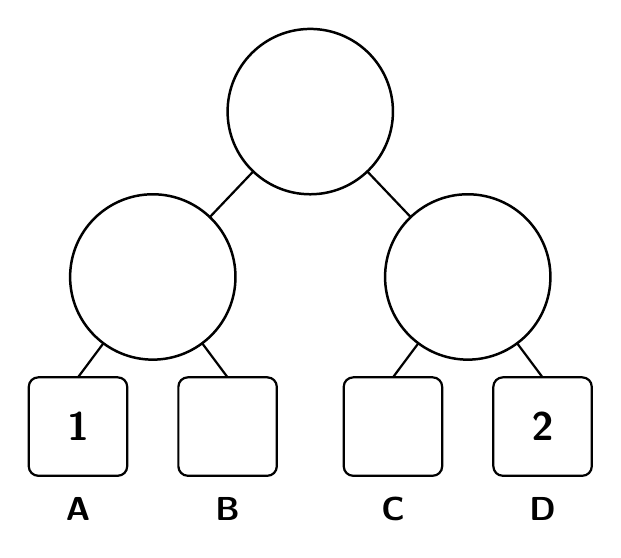
\begin{tikzpicture}[x=1mm,y=1mm,baseline=0]
\draw[line width=0.9pt] (0,0) circle (10.5);
\draw[line width=0.9pt] (-20,-21) circle (10.5);
\draw[line width=0.8pt] (-7.24,-7.60) -- (-12.76,-13.40);
\draw[line width=0.8pt] (-26.27,-29.42) -- (-29.50,-33.75);
\draw[line width=0.8pt, rounded corners=1.2mm] (-35.75,-46.25) rectangle (-23.25,-33.75);
\node[font=\bfseries\large] at (-29.50,-50.45) {A};
\node[font=\bfseries\Large] at (-29.50,-40.00) {1};
\draw[line width=0.8pt] (-13.73,-29.42) -- (-10.50,-33.75);
\draw[line width=0.8pt, rounded corners=1.2mm] (-16.75,-46.25) rectangle (-4.25,-33.75);
\node[font=\bfseries\large] at (-10.50,-50.45) {B};
\draw[line width=0.9pt] (20,-21) circle (10.5);
\draw[line width=0.8pt] (7.24,-7.60) -- (12.76,-13.40);
\draw[line width=0.8pt] (13.73,-29.42) -- (10.50,-33.75);
\draw[line width=0.8pt, rounded corners=1.2mm] (4.25,-46.25) rectangle (16.75,-33.75);
\node[font=\bfseries\large] at (10.50,-50.45) {C};
\draw[line width=0.8pt] (26.27,-29.42) -- (29.50,-33.75);
\draw[line width=0.8pt, rounded corners=1.2mm] (23.25,-46.25) rectangle (35.75,-33.75);
\node[font=\bfseries\large] at (29.50,-50.45) {D};
\node[font=\bfseries\Large] at (29.50,-40.00) {2};
\end{tikzpicture}\hspace{24mm}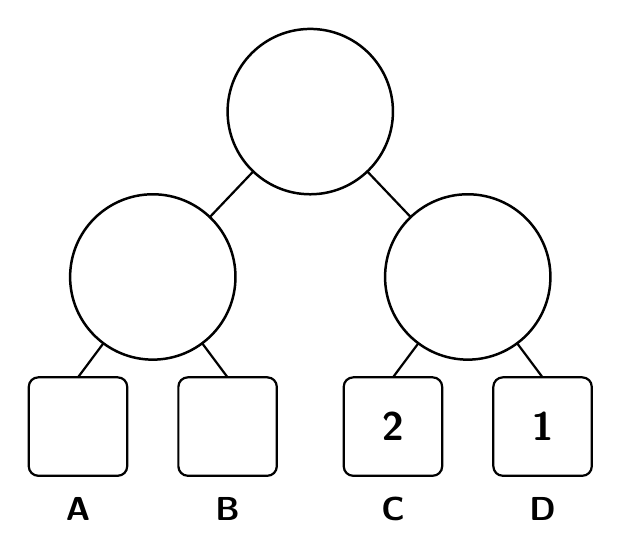
\begin{tikzpicture}[x=1mm,y=1mm,baseline=0]
\draw[line width=0.9pt] (0,0) circle (10.5);
\draw[line width=0.9pt] (-20,-21) circle (10.5);
\draw[line width=0.8pt] (-7.24,-7.60) -- (-12.76,-13.40);
\draw[line width=0.8pt] (-26.27,-29.42) -- (-29.50,-33.75);
\draw[line width=0.8pt, rounded corners=1.2mm] (-35.75,-46.25) rectangle (-23.25,-33.75);
\node[font=\bfseries\large] at (-29.50,-50.45) {A};
\draw[line width=0.8pt] (-13.73,-29.42) -- (-10.50,-33.75);
\draw[line width=0.8pt, rounded corners=1.2mm] (-16.75,-46.25) rectangle (-4.25,-33.75);
\node[font=\bfseries\large] at (-10.50,-50.45) {B};
\draw[line width=0.9pt] (20,-21) circle (10.5);
\draw[line width=0.8pt] (7.24,-7.60) -- (12.76,-13.40);
\draw[line width=0.8pt] (13.73,-29.42) -- (10.50,-33.75);
\draw[line width=0.8pt, rounded corners=1.2mm] (4.25,-46.25) rectangle (16.75,-33.75);
\node[font=\bfseries\large] at (10.50,-50.45) {C};
\node[font=\bfseries\Large] at (10.50,-40.00) {2};
\draw[line width=0.8pt] (26.27,-29.42) -- (29.50,-33.75);
\draw[line width=0.8pt, rounded corners=1.2mm] (23.25,-46.25) rectangle (35.75,-33.75);
\node[font=\bfseries\large] at (29.50,-50.45) {D};
\node[font=\bfseries\Large] at (29.50,-40.00) {1};
\end{tikzpicture}\hfill\null

\vspace{20mm}
\noindent\hfill 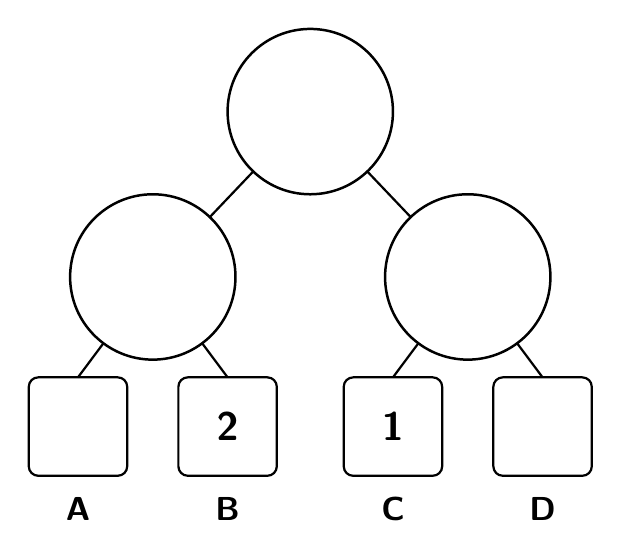
\begin{tikzpicture}[x=1mm,y=1mm,baseline=0]
\draw[line width=0.9pt] (0,0) circle (10.5);
\draw[line width=0.9pt] (-20,-21) circle (10.5);
\draw[line width=0.8pt] (-7.24,-7.60) -- (-12.76,-13.40);
\draw[line width=0.8pt] (-26.27,-29.42) -- (-29.50,-33.75);
\draw[line width=0.8pt, rounded corners=1.2mm] (-35.75,-46.25) rectangle (-23.25,-33.75);
\node[font=\bfseries\large] at (-29.50,-50.45) {A};
\draw[line width=0.8pt] (-13.73,-29.42) -- (-10.50,-33.75);
\draw[line width=0.8pt, rounded corners=1.2mm] (-16.75,-46.25) rectangle (-4.25,-33.75);
\node[font=\bfseries\large] at (-10.50,-50.45) {B};
\node[font=\bfseries\Large] at (-10.50,-40.00) {2};
\draw[line width=0.9pt] (20,-21) circle (10.5);
\draw[line width=0.8pt] (7.24,-7.60) -- (12.76,-13.40);
\draw[line width=0.8pt] (13.73,-29.42) -- (10.50,-33.75);
\draw[line width=0.8pt, rounded corners=1.2mm] (4.25,-46.25) rectangle (16.75,-33.75);
\node[font=\bfseries\large] at (10.50,-50.45) {C};
\node[font=\bfseries\Large] at (10.50,-40.00) {1};
\draw[line width=0.8pt] (26.27,-29.42) -- (29.50,-33.75);
\draw[line width=0.8pt, rounded corners=1.2mm] (23.25,-46.25) rectangle (35.75,-33.75);
\node[font=\bfseries\large] at (29.50,-50.45) {D};
\end{tikzpicture}\hspace{24mm}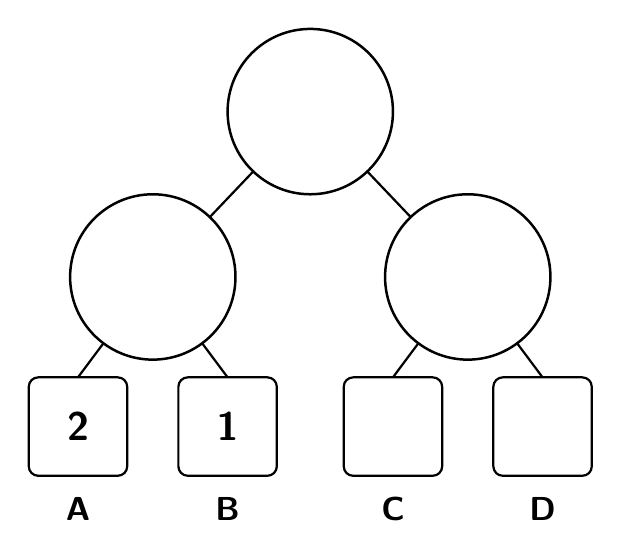
\begin{tikzpicture}[x=1mm,y=1mm,baseline=0]
\draw[line width=0.9pt] (0,0) circle (10.5);
\draw[line width=0.9pt] (-20,-21) circle (10.5);
\draw[line width=0.8pt] (-7.24,-7.60) -- (-12.76,-13.40);
\draw[line width=0.8pt] (-26.27,-29.42) -- (-29.50,-33.75);
\draw[line width=0.8pt, rounded corners=1.2mm] (-35.75,-46.25) rectangle (-23.25,-33.75);
\node[font=\bfseries\large] at (-29.50,-50.45) {A};
\node[font=\bfseries\Large] at (-29.50,-40.00) {2};
\draw[line width=0.8pt] (-13.73,-29.42) -- (-10.50,-33.75);
\draw[line width=0.8pt, rounded corners=1.2mm] (-16.75,-46.25) rectangle (-4.25,-33.75);
\node[font=\bfseries\large] at (-10.50,-50.45) {B};
\node[font=\bfseries\Large] at (-10.50,-40.00) {1};
\draw[line width=0.9pt] (20,-21) circle (10.5);
\draw[line width=0.8pt] (7.24,-7.60) -- (12.76,-13.40);
\draw[line width=0.8pt] (13.73,-29.42) -- (10.50,-33.75);
\draw[line width=0.8pt, rounded corners=1.2mm] (4.25,-46.25) rectangle (16.75,-33.75);
\node[font=\bfseries\large] at (10.50,-50.45) {C};
\draw[line width=0.8pt] (26.27,-29.42) -- (29.50,-33.75);
\draw[line width=0.8pt, rounded corners=1.2mm] (23.25,-46.25) rectangle (35.75,-33.75);
\node[font=\bfseries\large] at (29.50,-50.45) {D};
\end{tikzpicture}\hfill\null

\end{document}
